\documentclass[10pt]{article}

% ============================================================
% PACKAGES
% ============================================================

\usepackage[a4paper,margin=0.65in]{geometry}
\usepackage{amsmath,amssymb}
\usepackage{graphicx}
\usepackage{booktabs}
\usepackage{array}
\usepackage{float}
\usepackage{hyperref}
\usepackage{enumitem}
\usepackage{xcolor}
\usepackage{tikz}
\usepackage{multirow}
\usepackage{caption}
\usepackage{subcaption}
\usepackage{longtable}

\usetikzlibrary{
positioning,
arrows.meta,
shapes.geometric,
fit,
calc
}

% ============================================================
% FORMATTING
% ============================================================

\setlist{nosep,leftmargin=*}
\renewcommand{\arraystretch}{1.2}
\setlength{\parindent}{0pt}
\setlength{\parskip}{2pt}

\hypersetup{
    colorlinks=true,
    linkcolor=blue,
    urlcolor=blue,
    citecolor=blue
}

% ============================================================
% TIKZ STYLES
% ============================================================

\tikzset{
block/.style={
draw,
rounded corners,
minimum width=1.55cm,
minimum height=0.60cm,
align=center,
fill=blue!10,
font=\scriptsize
},
attn/.style={
draw,
rounded corners,
minimum width=1.55cm,
minimum height=0.60cm,
align=center,
fill=green!12,
font=\scriptsize
},
arrow/.style={
-{Latex[length=2mm]},
thin
}
}

% ============================================================
% DOCUMENT
% ============================================================

\begin{document}

% ============================================================
% TITLE
% ============================================================

\begin{center}

{\large\textbf{Shiv Nadar University Chennai}}\\[2mm]

{\normalsize\textbf{CS3807 -- Deep Learning Laboratory}}\\[2mm]

{\large\textbf{Experiments 8, 9}}\\[1mm]

{\normalsize
\textbf{
Effect of Attention Type and Attention Position\\
in a Pretrained ResNet50
}}

\end{center}

\vspace{3mm}

% ============================================================
% COURSE DETAILS
% ============================================================

\begin{center}
\begin{tabular}{|p{3.5cm}|p{8.7cm}|p{2.1cm}|}
\hline
\textbf{Degree \& Branch}
&
B.Tech Artificial Intelligence \& Data Science
&
Semester V
\\
\hline

\textbf{Subject Code \& Name}
&
CS3807 -- Deep Learning Laboratory
&
AY: 2026--27
\\
\hline
\end{tabular}
\end{center}

\vspace{4mm}
Name : Ashwin S\\
Reg no : 24011101007\\
Class : AI DS - A (batch 1)\\

% ============================================================
\section*{1. Objective}
% ============================================================

The objective of this experiment is to understand how different attention
mechanisms modify a pretrained convolutional neural network and how the
\textbf{position at which attention is inserted} influences image
classification performance.

A single pretrained architecture,

\[
\boxed{\text{ResNet50 pretrained on ImageNet}}
\]

is used throughout the experiment.

This report investigates:

\begin{itemize}

\item channel attention;

\item spatial attention;

\item sequential channel--spatial attention;

\item lightweight self-attention;

\item different positions for inserting attention within ResNet50;

\item single-stage and multi-stage attention;

\item attention ordering;

\item additional established attention mechanisms; and

\item qualitative interpretation using internal attention maps and Grad-CAM.

\end{itemize}

The experiment emphasizes that the effectiveness of attention depends not
only on the attention mechanism itself, but also on the characteristics of
the feature representation on which it operates.
\section*{2. Dataset}
% ============================================================

\textbf{Dataset: TensorFlow Flowers (\texttt{tf\_flowers})}

The TensorFlow Flowers dataset contains natural RGB flower images belonging
to five classes:

\begin{center}
\texttt{daisy},
\quad
\texttt{dandelion},
\quad
\texttt{roses},
\quad
\texttt{sunflowers},
\quad
\texttt{tulips}.
\end{center}

The images contain variations in:

\begin{itemize}

\item scale;

\item viewpoint;

\item illumination;

\item background clutter;

\item flower size;

\item color;

\item texture; and

\item object location.

\end{itemize}

These variations make the dataset suitable for studying the behavior of
attention mechanisms.

In this run, \texttt{tfds.load} could not be used on the Kaggle image because a
Protobuf version mismatch broke the \texttt{tensorflow\_datasets} import. The
data were therefore read from the official \texttt{flower\_photos} archive,
which is the same source that TFDS downloads for \texttt{tf\_flowers}. The
images and classes are identical, and the labels were mapped to the TFDS index
order (dandelion, daisy, tulips, sunflowers, roses). All 3{,}670 images were used.

\begin{figure}[H]
\centering
\includegraphics[width=0.78\textwidth]{figures/15_sample_images_all_classes.png}
\caption{Sample training images from all five classes after resizing to $224\times224\times3$.}
\end{figure}
\noindent The classes differ a lot in scale and framing,
from single close-up blooms to whole fields, and a few labels are clearly noisy (the tulip row contains a water fountain and a park scene with only a distant flowerbed). Such images carry little flower evidence for any model, so they put a ceiling on accuracy that attention alone cannot remove.

\subsection*{2.1 Image Preprocessing}
% ============================================================

Every input image was resized to

\[
224\times224\times3.
\]

The image was preprocessed using the preprocessing procedure expected
by the ImageNet-pretrained ResNet50.

The data augmentation used included:

\begin{itemize}

\item random horizontal flipping;

\item small rotations;

\item random zoom;

\item random translation; and

\item mild contrast variation.

\end{itemize}

The same augmentation strategy was maintained for all model comparisons.

Each image was resized directly to $224\times224$ with bilinear
interpolation (the aspect ratio is not preserved) and then passed through the
ResNet50 ``caffe'' preprocessing (RGB$\rightarrow$BGR and ImageNet mean
subtraction). I checked that this gives exactly the same output as
\texttt{keras.applications.resnet50.preprocess\_input}. The augmentation used
for every model was a random horizontal flip, a rotation of up to
$\pm18^\circ$, zoom and translation of up to $\pm10\%$, and a contrast change of
up to $\pm10\%$. It was applied only to training images and re-created with the
same seed (42) at the start of every run.

\subsection*{2.2 Dataset Split}
% ============================================================

The same training, validation, and testing split was used for every experiment:

\[
\boxed{
70\% : 15\% : 15\%
}
\]

for

\[
\text{Training : Validation : Testing}.
\]

The exact same samples were retained in each subset for all ablation
experiments.

This was necessary to ensure that differences in performance are caused by
changes in the model rather than changes in the dataset split.

The split was stratified by class with a fixed seed (42). The selected indices
(with source file names) were saved once and reused by all seventeen trained
models, giving the following subsets:

\begin{center}
\begin{tabular}{|l|c|c|c|c|}
\hline
\textbf{Class} & \textbf{Train} & \textbf{Validation} & \textbf{Test} & \textbf{Total}\\
\hline
dandelion & 629 & 134 & 135 & 898\\
daisy & 443 & 95 & 95 & 633\\
tulips & 559 & 120 & 120 & 799\\
sunflowers & 489 & 105 & 105 & 699\\
roses & 449 & 96 & 96 & 641\\
\hline
\textbf{Total} & \textbf{2569} & \textbf{550} & \textbf{551} & \textbf{3670}\\
\hline
\end{tabular}
\end{center}

\section*{3. Pretrained Architecture: ResNet50}
% ============================================================

ResNet50 pretrained using ImageNet is used as the
\textbf{only backbone architecture} in this experiment.

For an input image

\[
I\in\mathbb{R}^{224\times224\times3},
\]

the major ResNet50 stages produce approximately the following feature
dimensions:

\begin{center}

\begin{tabular}{|l|c|c|}
\hline
\textbf{ResNet50 Stage}
&
\textbf{Spatial Resolution}
&
\textbf{Channels}
\\
\hline

Stem + MaxPool
&
$56\times56$
&
64
\\
\hline

conv2\_x
&
$56\times56$
&
256
\\
\hline

conv3\_x
&
$28\times28$
&
512
\\
\hline

conv4\_x
&
$14\times14$
&
1024
\\
\hline

conv5\_x
&
$7\times7$
&
2048
\\
\hline

\end{tabular}

\end{center}

As the network becomes deeper:

\[
\boxed{
\text{Spatial Resolution}\downarrow
}
\]

while

\[
\boxed{
\text{Feature Channels}\uparrow
}
\]

and the representation generally progresses from low-level visual
information toward higher-level semantic information.

Keras' built-in ResNet50 does not allow a layer to be inserted between two
stages, so the network was rebuilt layer by layer with the same layer names and
the ImageNet weights were copied into it. The rebuilt backbone reproduced the
reference model exactly (maximum absolute output difference $0.000$), has
23{,}587{,}712 parameters without the classification top, and gave the stage
dimensions listed above.

\section*{4. Understanding ResNet50 Feature Hierarchy}
% ============================================================

The approximate interpretation of different stages is:

\begin{itemize}

\item \textbf{Early features:}
edges, colors, orientations, boundaries, and simple textures.

\item \textbf{Intermediate features:}
local patterns, repeated structures, flower parts, petal arrangements, and
shape information.

\item \textbf{Late features:}
high-level object structures and class-discriminative semantic information.

\end{itemize}

Therefore, the same attention mechanism may produce different behavior when
inserted at different locations.
\section*{5. Why Attention Position Matters}
% ============================================================

Attention is not independent of the features on which it operates.

Suppose an attention module receives

\[
F\in\mathbb{R}^{H\times W\times C}.
\]

The values of

\[
H,\qquad W,\qquad C
\]

and the semantic meaning of the feature tensor change significantly with
network depth.

Therefore:

\begin{itemize}

\item \textbf{early-stage attention} operates on high-resolution,
low-level visual information;

\item \textbf{middle-stage attention} operates on intermediate features
containing both spatial and semantic information; and

\item \textbf{late-stage attention} operates on low-resolution,
high-level semantic representations.

\end{itemize}

This report therefore investigates both:

\[
\boxed{\text{Which attention mechanism should be used?}}
\]

and

\[
\boxed{\text{Where should the attention mechanism be inserted?}}
\]
\section*{6. Candidate Attention Positions}
% ============================================================

Four candidate attention positions in ResNet50 are defined.

\[
P_1:
\text{ after conv2\_x},
\]

\[
P_2:
\text{ after conv3\_x},
\]

\[
P_3:
\text{ after conv4\_x},
\]

\[
P_4:
\text{ after conv5\_x}.
\]

The corresponding feature dimensions are:

\begin{center}

\begin{tabular}{|c|c|c|c|}
\hline

\textbf{Position}
&
\textbf{Location}
&
\textbf{Resolution}
&
\textbf{Channels}
\\
\hline

$P_1$
&
After conv2\_x
&
$56\times56$
&
256
\\
\hline

$P_2$
&
After conv3\_x
&
$28\times28$
&
512
\\
\hline

$P_3$
&
After conv4\_x
&
$14\times14$
&
1024
\\
\hline

$P_4$
&
After conv5\_x
&
$7\times7$
&
2048
\\
\hline

\end{tabular}

\end{center}

The principal laboratory exercise concentrates on

\[
\boxed{
P_2,\quad P_3,\quad P_4
}
\]

because $P_1$ contains comparatively high-resolution features and may
substantially increase the computational cost of some attention mechanisms.

$P_1$ was still evaluated once (model B1 in Main Experiment 2), because the
channel--spatial module is cheap there (8{,}563 parameters). Self-attention
was not placed at $P_1$, for the cost reason above.

\section*{7. Baseline Model}
% ============================================================

The baseline is the pretrained ResNet50 without any additional attention
mechanism.

\begin{center}

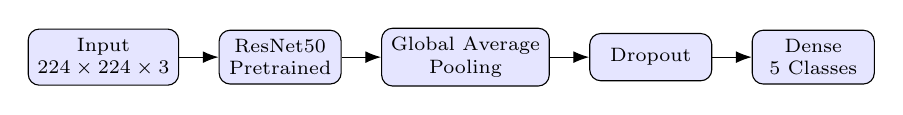
\begin{tikzpicture}[node distance=5mm]

\node[block] (a)
{Input\\$224\times224\times3$};

\node[block,right=of a] (b)
{ResNet50\\Pretrained};

\node[block,right=of b] (c)
{Global Average\\Pooling};

\node[block,right=of c] (d)
{Dropout};

\node[block,right=of d] (e)
{Dense\\5 Classes};

\foreach \x/\y in {a/b,b/c,c/d,d/e}
\draw[arrow] (\x)--(\y);

\end{tikzpicture}

\end{center}

The baseline establishes the reference performance against which the
attention-based models are compared.

In the implementation, the dropout rate was $0.3$. The dense layer produces
logits that go through a separate softmax, so the pre-softmax class score $y^c$
is available for Grad-CAM. The baseline has 23{,}597{,}957 parameters in total.

\section*{8. Channel Attention}
% ============================================================

Consider a feature tensor

\[
F\in\mathbb{R}^{H\times W\times C}.
\]

Channel attention determines the relative importance of different feature
channels.

Global average pooling is first used to generate a channel descriptor:

\[
z_c
=
\frac{1}{HW}
\sum_{i=1}^{H}
\sum_{j=1}^{W}
F(i,j,c).
\]

Thus,

\[
z\in\mathbb{R}^{C}.
\]

The channel descriptor is transformed using two learnable transformations:

\[
M_c(F)
=
\sigma
\left(
W_2
\delta
\left(
W_1z
\right)
\right),
\]

where:

\begin{itemize}

\item $\delta(\cdot)$ denotes a nonlinear activation such as ReLU;

\item $\sigma(\cdot)$ denotes the sigmoid activation;

\item $W_1$ reduces the channel representation; and

\item $W_2$ restores the channel dimension.

\end{itemize}

The refined feature tensor is:

\[
F_c
=
F\odot M_c(F).
\]

Channel attention attempts to answer:

\[
\boxed{\text{Which feature channels are important?}}
\]

A reduction ratio of

\[
r=16
\]

was used as the default setting throughout the laboratory experiment.

The reduction ratio was not treated as a separate mandatory ablation.

$r=16$ was used in every model. With this setting the module is exactly the
Squeeze-and-Excitation block, so the ``Channel / SE'' entry of the additional
comparison reuses this model (A1) instead of training an identical copy. At
$P_3$ it adds 132{,}160 parameters.

\section*{9. Spatial Attention}
% ============================================================

Spatial attention determines the spatial regions that should receive greater
importance.

For the input feature tensor

\[
F\in\mathbb{R}^{H\times W\times C},
\]

compute average pooling across channels:

\[
F_{\mathrm{avg}}
=
\operatorname{Mean}_{c}(F),
\]

and maximum pooling across channels:

\[
F_{\mathrm{max}}
=
\operatorname{Max}_{c}(F).
\]

Both tensors have dimensions

\[
H\times W\times1.
\]

Concatenate them:

\[
F_s
=
[
F_{\mathrm{avg}}
\Vert
F_{\mathrm{max}}
].
\]

The spatial attention map is then computed as

\[
M_s(F)
=
\sigma
\left(
\operatorname{Conv}_{7\times7}(F_s)
\right).
\]

Therefore,

\[
M_s(F)
\in
\mathbb{R}^{H\times W\times1}.
\]

The spatially refined feature is

\[
F_s'
=
F\odot M_s(F).
\]

Spatial attention answers:

\[
\boxed{\text{Which spatial locations are important?}}
\]

The $7\times7$ kernel was used for every model except Main Experiment 5. The
module adds only 99 parameters ($2\times7\times7$ weights plus a bias),
whatever the position.

\section*{10. Sequential Channel--Spatial Attention}
% ============================================================

Channel and spatial attention can be sequentially applied.

First,

\[
F_c
=
M_c(F)\odot F.
\]

Then,

\[
F_{cs}
=
M_s(F_c)\odot F_c.
\]

The overall structure becomes:

\[
\boxed{
F
\rightarrow
\text{Channel Attention}
\rightarrow
\text{Spatial Attention}
\rightarrow
F_{cs}
}
\]

This arrangement first determines

\[
\text{``what is important''}
\]

and then determines

\[
\text{``where it is important.''}
\]

A simplified diagram is shown below.

\begin{center}

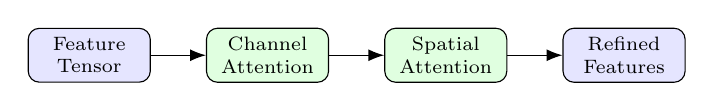
\begin{tikzpicture}[node distance=7mm]

\node[block] (a)
{Feature\\Tensor};

\node[attn,right=of a] (b)
{Channel\\Attention};

\node[attn,right=of b] (c)
{Spatial\\Attention};

\node[block,right=of c] (d)
{Refined\\Features};

\draw[arrow] (a)--(b);
\draw[arrow] (b)--(c);
\draw[arrow] (c)--(d);

\end{tikzpicture}

\end{center}
\section*{11. Self-Attention}
% ============================================================

Self-attention allows spatial locations to interact directly with other
spatial locations.

For

\[
F\in\mathbb{R}^{H\times W\times C},
\]

flatten the spatial dimensions:

\[
X\in\mathbb{R}^{N\times C},
\]

where

\[
N=HW.
\]

Generate the query, key, and value matrices:

\[
Q=XW_Q,
\]

\[
K=XW_K,
\]

and

\[
V=XW_V.
\]

The attention matrix is

\[
A
=
\operatorname{softmax}
\left(
\frac{QK^T}{\sqrt{d}}
\right),
\]

where $d$ is the dimension of the query/key representation.

The attended output is

\[
Y=AV.
\]

After reshaping the output back to the original spatial structure, a residual
formulation is used:

\[
F_{\mathrm{SA}}
=
F
+
\gamma
\operatorname{reshape}(Y),
\]

where $\gamma$ is a learnable scaling parameter.

Self-attention attempts to answer:

\[
\boxed{
\text{Which spatial features are related to other spatial features?}
}
\]

Since the attention matrix has dimension approximately

\[
N\times N,
\]

its computational requirements increase rapidly as

\[
N=HW
\]

increases.

Therefore, self-attention was preferably introduced at

\[
P_3
\]

or

\[
P_4.
\]

In the implementation, $W_Q$, $W_K$ and $W_V$ are $1\times1$ convolutions. The
query and key use $d=C/8$ (128 at $P_3$), the value keeps all $C$ channels, and
$\gamma$ starts at zero so that the module begins as an identity mapping. The
layer also returns $A$, but only for visualisation. At $P_3$ the module adds
1{,}312{,}001 parameters. The size of $A$ at each position shows why
$P_3$/$P_4$ are preferred:

\begin{center}
\begin{tabular}{|c|c|c|c|c|}
\hline
\textbf{Position} & \textbf{Resolution} & $N=HW$ & \textbf{Size of $A$} & \textbf{Memory / image (float32)}\\
\hline
$P_1$ & $56\times56$ & 3136 & $3136\times3136$ & 37.52 MB\\
$P_2$ & $28\times28$ & 784 & $784\times784$ & 2.34 MB\\
$P_3$ & $14\times14$ & 196 & $196\times196$ & 0.147 MB\\
$P_4$ & $7\times7$ & 49 & $49\times49$ & 0.009 MB\\
\hline
\end{tabular}
\end{center}

\section*{12. Inserting Attention into ResNet50}
% ============================================================

For any selected stage $P_k$, the network structure can be written as

\[
\text{Previous ResNet Stage}
\rightarrow
\text{Attention}
\rightarrow
\text{Next ResNet Stage}.
\]

For example, attention inserted after conv4\_x gives:

\[
\boxed{
\text{conv4\_x}
\rightarrow
\text{Attention}
\rightarrow
\text{conv5\_x}
}
\]

For channel--spatial attention:

\[
\boxed{
\text{conv4\_x}
\rightarrow
\text{Channel Attention}
\rightarrow
\text{Spatial Attention}
\rightarrow
\text{conv5\_x}
}
\]

The feature dimensions immediately before and after
the attention block were recorded for every model.

Attention does not unintentionally modify the spatial or channel
dimensions unless the selected mechanism explicitly requires such a
transformation.

The dimensions recorded immediately before and after every attention block are
given below. No module changed the shape of the tensor it received.

\begin{center}
\resizebox{\textwidth}{!}{
\begin{tabular}{|l|l|c|l|c|c|}
\hline
\textbf{Model} & \textbf{Attention} & \textbf{Position} & \textbf{Placement} & \textbf{Input $(H,W,C)$} & \textbf{Output $(H,W,C)$}\\
\hline
A1, A2, A3, A4, A5 & Channel / Spatial / C$\rightarrow$S / SA / C$\rightarrow$S$\rightarrow$SA & $P_3$ & conv4\_x $\rightarrow$ Attention $\rightarrow$ conv5\_x & (14, 14, 1024) & (14, 14, 1024)\\
B1 & Channel$\rightarrow$Spatial & $P_1$ & conv2\_x $\rightarrow$ Attention $\rightarrow$ conv3\_x & (56, 56, 256) & (56, 56, 256)\\
B2 & Channel$\rightarrow$Spatial & $P_2$ & conv3\_x $\rightarrow$ Attention $\rightarrow$ conv4\_x & (28, 28, 512) & (28, 28, 512)\\
B4 & Channel$\rightarrow$Spatial & $P_4$ & conv5\_x $\rightarrow$ Attention $\rightarrow$ GAP & (7, 7, 2048) & (7, 7, 2048)\\
$P_3+P_4$ & Channel$\rightarrow$Spatial & $P_3$, $P_4$ & both placements above & (14,14,1024), (7,7,2048) & unchanged\\
$P_2+P_3+P_4$ & Channel$\rightarrow$Spatial & $P_2$, $P_3$, $P_4$ & all three placements & (28,28,512), (14,14,1024), (7,7,2048) & unchanged\\
O\_SC, K3, K5 & S$\rightarrow$C, C$\rightarrow$S ($k=3$), C$\rightarrow$S ($k=5$) & $P_3$ & conv4\_x $\rightarrow$ Attention $\rightarrow$ conv5\_x & (14, 14, 1024) & (14, 14, 1024)\\
ECA, CBAM, COORD & ECA / CBAM / Coordinate & $P_3$ & conv4\_x $\rightarrow$ Attention $\rightarrow$ conv5\_x & (14, 14, 1024) & (14, 14, 1024)\\
\hline
\end{tabular}}
\end{center}

\section*{13. Main Experiment 1: Attention-Type Ablation}
% ============================================================

The first experiment studies the effect of different types of attention.

The attention position was fixed at

\[
\boxed{
P_3=\text{after conv4\_x}
}
\]

for all models.

The following were compared:

\begin{center}

\begin{tabular}{|l|c|c|c|}
\hline

\textbf{Model}
&
\textbf{Channel}
&
\textbf{Spatial}
&
\textbf{Self-Attention}
\\
\hline

A0: Baseline ResNet50
&
--
&
--
&
--
\\
\hline

A1: Channel Attention
&
$\checkmark$
&
--
&
--
\\
\hline

A2: Spatial Attention
&
--
&
$\checkmark$
&
--
\\
\hline

A3: Channel+Spatial
&
$\checkmark$
&
$\checkmark$
&
--
\\
\hline

A4: Self-Attention
&
--
&
--
&
$\checkmark$
\\
\hline

A5: Combined Attention
&
$\checkmark$
&
$\checkmark$
&
$\checkmark$
\\
\hline

\end{tabular}

\end{center}

This experiment investigates:

\[
\boxed{
\text{How does attention type affect model performance?}
}
\]

The following were kept identical:

\begin{itemize}

\item dataset split;

\item preprocessing;

\item augmentation;

\item optimizer;

\item learning rate schedule;

\item epochs;

\item batch size;

\item backbone;

\item classifier;

\item attention position; and

\item evaluation procedure.

\end{itemize}

\subsection*{13.1 Results}

All six models were trained and evaluated under the protocol of Section 19
(Transfer-Learning Strategy).

\begin{center}
\resizebox{\textwidth}{!}{
\begin{tabular}{|l|c|c|c|c|c|c|c|}
\hline
\textbf{Model} & \textbf{Accuracy} & \textbf{Precision} & \textbf{Recall} & \textbf{Macro F1} & \textbf{Attention Params} & \textbf{Inference (ms/img)} & \textbf{Best Val Acc (epoch)}\\
\hline
A0: Baseline ResNet50 & 0.9292 & 0.9282 & 0.9274 & 0.9277 & 0 & 9.38 & 0.9327 (17)\\
A1: Channel Attention & 0.9256 & 0.9262 & 0.9223 & 0.9237 & 132{,}160 & 9.70 & 0.9364 (20)\\
A2: Spatial Attention & 0.9310 & 0.9336 & 0.9267 & 0.9295 & 99 & 9.72 & 0.9291 (17)\\
A3: Channel+Spatial & \textbf{0.9328} & 0.9326 & \textbf{0.9296} & \textbf{0.9309} & 132{,}259 & 9.81 & 0.9400 (14)\\
A4: Self-Attention & 0.9002 & 0.8999 & 0.8972 & 0.8981 & 1{,}312{,}001 & 9.89 & 0.9382 (4)\\
A5: Combined Attention & \textbf{0.9328} & \textbf{0.9345} & 0.9282 & 0.9308 & 1{,}444{,}260 & 9.87 & 0.9400 (12)\\
\hline
\end{tabular}}
\end{center}

A3 and A5 tie for the best accuracy at 0.9328, which is 514 of 551 test images
correct against 512 for the baseline. Spatial attention alone is one image ahead
of the baseline, and channel attention alone is two images behind it. So the
first four rows sit within a band of about four images, and with a single seed
I would not read a strong ranking into that band.

Self-attention is the one clear outlier, 16 images below the baseline. Its
selected checkpoint came from epoch 4, which is still in the frozen-backbone
phase: validation accuracy peaked very early (0.9382) and never beat that
during fine-tuning, so the test model never benefited from conv5\_x
fine-tuning. A5 adds the same self-attention block but on top of
channel$\rightarrow$spatial features, and it did not show this early peak.
Training curves, bar graphs and confusion matrices for these models are
analysed in Sections 22 and 23.

\section*{14. Main Experiment 2: Attention-Position Ablation}
% ============================================================

The second experiment investigates the influence of the position of
attention.

The attention type was fixed as:

\[
\boxed{
\text{Channel Attention}
\rightarrow
\text{Spatial Attention}
}
\]

and the same module was inserted at different stages.

\begin{center}

\begin{tabular}{|l|l|c|c|}
\hline

\textbf{Experiment}
&
\textbf{Attention Position}
&
\textbf{Resolution}
&
\textbf{Channels}
\\
\hline

B1
&
After conv2\_x
&
$56\times56$
&
256
\\
\hline

B2
&
After conv3\_x
&
$28\times28$
&
512
\\
\hline

B3
&
After conv4\_x
&
$14\times14$
&
1024
\\
\hline

B4
&
After conv5\_x
&
$7\times7$
&
2048
\\
\hline

\end{tabular}

\end{center}

The results shed light on whether attention is more beneficial for:

\begin{itemize}

\item high-resolution low-level features;

\item intermediate representations; or

\item low-resolution semantic features.

\end{itemize}

The principal question is:

\[
\boxed{
\text{How does the location of attention influence performance?}
}
\]

\subsection*{14.1 Results}

B3 is the same configuration as A3 (Channel$\rightarrow$Spatial at $P_3$,
$k=7$), so that trained model was reused rather than retrained.

\begin{center}
\resizebox{\textwidth}{!}{
\begin{tabular}{|l|l|c|c|c|c|c|c|c|c|}
\hline
\textbf{Exp.} & \textbf{Position} & \textbf{Resolution} & \textbf{Channels} & \textbf{Accuracy} & \textbf{Precision} & \textbf{Recall} & \textbf{Macro F1} & \textbf{Attention Params} & \textbf{Inference (ms/img)}\\
\hline
A0 (reference) & -- & -- & -- & 0.9292 & 0.9282 & 0.9274 & 0.9277 & 0 & 9.38\\
B1 & After conv2\_x ($P_1$) & $56\times56$ & 256 & 0.8984 & 0.8971 & 0.8983 & 0.8970 & 8{,}563 & 9.62\\
B2 & After conv3\_x ($P_2$) & $28\times28$ & 512 & 0.9238 & 0.9222 & 0.9223 & 0.9221 & 33{,}411 & 9.63\\
B3 & After conv4\_x ($P_3$) & $14\times14$ & 1024 & \textbf{0.9328} & \textbf{0.9326} & \textbf{0.9296} & \textbf{0.9309} & 132{,}259 & 9.81\\
B4 & After conv5\_x ($P_4$) & $7\times7$ & 2048 & 0.9256 & 0.9276 & 0.9225 & 0.9246 & 526{,}563 & 9.79\\
\hline
\end{tabular}}
\end{center}

Performance rises from $P_1$ to a peak at $P_3$ and then falls again at $P_4$.
Only the $P_3$ placement beats the baseline. The early placements suffer most,
and the reason is probably the training setup: during phase 1 every ResNet
stage after the module is frozen, so conv3\_x--conv5\_x keep receiving
re-weighted features they were never trained on, and only conv5\_x is later
allowed to adapt. B2 shows this clearly, with only 0.6291 validation accuracy
after its first epoch against about 0.86 for the baseline.

At $P_4$ the module sits right before global pooling and has 527K trainable
parameters. It fit the training set quickly (training accuracy 0.983 already at
epoch 10) while its validation loss drifted up to 0.36, which looks like
overfitting rather than a lack of capacity. The spatial maps at the different
positions are compared in Section 27.

\section*{15. Main Experiment 3: Multiple Attention Positions}
% ============================================================

Attention may also be inserted at more than one ResNet50 stage.

The following were compared:

\[
\text{Attention only at }P_3,
\]

\[
\text{Attention only at }P_4,
\]

and

\[
\text{Attention at }P_3+P_4.
\]

As an extended experiment, the following was also evaluated:

\[
P_2+P_3+P_4.
\]

The purpose is to investigate whether applying attention repeatedly provides
sufficient performance improvement to justify the additional:

\begin{itemize}

\item parameters;

\item computation;

\item memory;

\item training time; and

\item inference time.

\end{itemize}

The results below answer:

\[
\boxed{
\text{Is attention at more locations necessarily more effective?}
}
\]

\subsection*{15.1 Results}

``Only $P_3$'' reuses A3 and ``only $P_4$'' reuses B4. The two
multi-position models were trained separately. Computation was measured as
GFLOPs per image with the TensorFlow profiler, memory as the peak GPU memory
during training, and training time as the wall-clock time for all 20 epochs.

\begin{center}
\resizebox{\textwidth}{!}{
\begin{tabular}{|l|c|c|c|c|c|c|c|c|}
\hline
\textbf{Configuration} & \textbf{Accuracy} & \textbf{Precision} & \textbf{Recall} & \textbf{Macro F1} & \textbf{Attention Params} & \textbf{GFLOPs} & \textbf{Train Time (s)} & \textbf{Inference (ms/img)}\\
\hline
No attention (reference) & 0.9292 & 0.9282 & 0.9274 & 0.9277 & 0 & 7.7512 & 453.3 & 9.38\\
Only $P_3$ & \textbf{0.9328} & \textbf{0.9326} & \textbf{0.9296} & \textbf{0.9309} & 132{,}259 & 7.7523 & 461.2 & 9.81\\
Only $P_4$ & 0.9256 & 0.9276 & 0.9225 & 0.9246 & 526{,}563 & 7.7527 & 446.4 & 9.80\\
$P_3+P_4$ & 0.9111 & 0.9129 & 0.9088 & 0.9098 & 658{,}822 & 7.7538 & 456.8 & 9.64\\
$P_2+P_3+P_4$ (extended) & 0.9129 & 0.9088 & 0.9116 & 0.9097 & 692{,}233 & 7.7556 & 469.5 & 9.74\\
\hline
\end{tabular}}
\end{center}

\begin{figure}[H]
\centering
\includegraphics[width=0.70\textwidth]{figures/20_exp3_multiple_positions_performance.png}
\caption{Experiment 3: accuracy and macro F1 for single and multiple attention positions.}
\end{figure}
\noindent A single module at $P_3$ is the best configuration, and every additional
placement makes things worse: $P_3+P_4$ and $P_2+P_3+P_4$ both fall about 1.6--1.8
points below even the plain baseline. Stacking modules gives a frozen backbone
more freshly initialised layers to adapt to at once, and the $P_3+P_4$ model ended
with the highest validation loss of all runs (0.536) at a training loss of 0.010,
a clear overfitting signature.


\begin{figure}[H]
\centering
\includegraphics[width=\textwidth]{figures/21_exp3_multiple_positions_complexity.png}
\caption{Experiment 3: attention parameters, GFLOPs, training time, peak training GPU memory and inference time.}
\end{figure}
\noindent Attention parameters grow from 132K to 692K, almost entirely because of the
2048-channel module at $P_4$, yet GFLOPs barely move (7.7512 to 7.7556) and
training and inference times stay within a few percent. Peak memory rises with
the number of positions (1{,}849 MB for $P_3$ only to 3{,}831 MB for three
positions). The baseline's 3{,}224 MB, however, shows that this number also
reflects how TensorFlow's allocator happened to reserve memory, so I treat it as
rough. The extra cost is small, but it buys no accuracy, so more positions are not
worth it here.

\section*{16. Main Experiment 4: Attention Order}
% ============================================================

The sequence in which channel and spatial attention are applied may influence
the resulting features.

The following were compared:

\[
\boxed{
\text{Channel}
\rightarrow
\text{Spatial}
}
\]

against

\[
\boxed{
\text{Spatial}
\rightarrow
\text{Channel}
}
\]

while maintaining the same insertion position.

For example, at $P_3$:

\[
F
\rightarrow
M_c
\rightarrow
M_s
\]

was compared with

\[
F
\rightarrow
M_s
\rightarrow
M_c.
\]

The results determine whether selecting informative feature channels
before selecting spatial regions produces behavior different from selecting
spatial regions first.

\subsection*{16.1 Results}

The Channel$\rightarrow$Spatial model is A3 (reused). Spatial$\rightarrow$Channel was
trained with the identical module, position, kernel and protocol.

\begin{center}
\resizebox{\textwidth}{!}{
\begin{tabular}{|l|c|c|c|c|c|c|c|c|}
\hline
\textbf{Order at $P_3$} & \textbf{Accuracy} & \textbf{Precision} & \textbf{Recall} & \textbf{Macro F1} & \textbf{Attention Params} & \textbf{Inference (ms/img)} & \textbf{Best Val Acc (epoch)} & \textbf{Final Val Loss}\\
\hline
No attention (reference) & 0.9292 & 0.9282 & 0.9274 & 0.9277 & 0 & 9.38 & 0.9327 (17) & 0.3087\\
Channel$\rightarrow$Spatial ($F\rightarrow M_c\rightarrow M_s$) & \textbf{0.9328} & \textbf{0.9326} & 0.9296 & \textbf{0.9309} & 132{,}259 & 9.81 & 0.9400 (14) & 0.3311\\
Spatial$\rightarrow$Channel ($F\rightarrow M_s\rightarrow M_c$) & 0.9310 & 0.9304 & 0.9296 & 0.9300 & 132{,}259 & 9.89 & 0.9255 (15) & 0.4183\\
\hline
\end{tabular}}
\end{center}

\begin{figure}[H]
\centering
\includegraphics[width=0.70\textwidth]{figures/22_exp4_attention_order_metrics.png}
\caption{Experiment 4: accuracy, precision, recall and macro F1 for the two attention orders.}
\end{figure}
\noindent The two orders end up practically tied: Channel$\rightarrow$Spatial is
ahead by one test image in accuracy, and recall is identical (0.9296). On final
test numbers alone the order does not matter in this setup, since the gap is
smaller than what a different seed could produce.


\begin{figure}[H]
\centering
\includegraphics[width=0.85\textwidth]{figures/23_exp4_attention_order_spatial_maps.png}
\caption{Experiment 4: spatial-attention maps and overlays for Channel$\rightarrow$Spatial and Spatial$\rightarrow$Channel.}
\end{figure}
\noindent Both orders learn border-shaped maps that stay close to 1 inside the image,
but the Spatial$\rightarrow$Channel maps have a much narrower range: their lowest
values are around 0.5--0.8, against about 0.15--0.2 for Channel$\rightarrow$Spatial.
When the spatial gate acts first, on raw conv4\_x features, it suppresses far less.
That order also trained more awkwardly, with 0.18 validation accuracy after
epoch 1 (close to chance) and a higher final validation loss (0.418 vs 0.331).
So order changed the training behaviour more than the final score.

\section*{17. Main Experiment 5: Spatial Attention Kernel Size}
% ============================================================

The receptive field used to generate the spatial attention map may influence
the result.

The following were evaluated:

\[
k\in\{3,5,7\}.
\]

The same attention position and training protocol were used.

\begin{center}
\resizebox{\textwidth}{!}{
\begin{tabular}{|c|c|c|c|c|c|}
\hline
\textbf{Spatial Kernel} & \textbf{Accuracy} & \textbf{Macro F1} & \textbf{Inference Time (ms/img)} & \textbf{Attention Params} & \textbf{Best Val Acc (epoch)}\\
\hline
$3\times3$ & \textbf{0.9328} & \textbf{0.9309} & 9.63 & 132{,}179 & 0.9327 (19)\\
\hline
$5\times5$ & 0.9274 & 0.9259 & 9.73 & 132{,}211 & 0.9273 (17)\\
\hline
$7\times7$ & \textbf{0.9328} & \textbf{0.9309} & 9.81 & 132{,}259 & 0.9400 (14)\\
\hline
\end{tabular}}
\end{center}

The results below address whether a larger spatial kernel provides a useful
increase in contextual information.

All three runs use Channel$\rightarrow$Spatial at $P_3$; the $7\times7$ run is A3
(reused). The $3\times3$ and $7\times7$ models reached exactly the same test
accuracy, precision, recall and macro F1, even though they selected different
checkpoints, while $5\times5$ was three images behind.

\begin{figure}[H]
\centering
\includegraphics[width=0.85\textwidth]{figures/24_exp5_kernel_size_metrics.png}
\caption{Experiment 5: performance and inference time against spatial-attention kernel size.}
\end{figure}
\noindent Accuracy is V-shaped (0.9328, 0.9274, 0.9328) rather than increasing with
$k$, while inference time creeps up from 9.63 to 9.81 ms. A larger receptive
field for the spatial gate does not buy accuracy here, so $3\times3$ gives the
same result as $7\times7$ for slightly less time and 80 fewer parameters.


\begin{figure}[H]
\centering
\includegraphics[width=0.92\textwidth]{figures/25_exp5_kernel_size_spatial_maps.png}
\caption{Experiment 5: spatial-attention maps and overlays for $k=3$, $5$ and $7$.}
\end{figure}
\noindent The kernel size changes the texture of the map more than its meaning. With
$k=3$ the low values are scattered as small patches through the interior (range
about 0.65--1). With $k=5$ they form a frame around all borders, and with $k=7$
they are smooth and limited to the left and bottom edges. A larger kernel gives a
smoother, more border-driven map, but none of them outlines the flower, which
explains why accuracy does not follow $k$.

\section*{18. Additional Task: Comparison of Different Attention Mechanisms}
% ============================================================

As an additional exploration task, the attention
mechanisms implemented in the laboratory are compared with established attention
approaches.

At least

\[
\boxed{\text{two additional attention mechanisms}}
\]

were selected from the following:

\begin{itemize}

\item Squeeze-and-Excitation (SE) Attention;

\item Efficient Channel Attention (ECA);

\item Convolutional Block Attention Module (CBAM);

\item Coordinate Attention; and

\item lightweight Self-Attention.

\end{itemize}

The pretrained backbone remains:

\[
\boxed{\text{ResNet50}}
\]

for all comparisons.

To ensure a fair comparison, the additional attention mechanisms were
inserted at the same position:

\[
\boxed{
P_3=\text{after conv4\_x}
}
\]

Five mechanisms from this list were compared at $P_3$: SE, ECA, CBAM,
Coordinate Attention and the lightweight self-attention. SE is identical to the
channel attention of Section 8 (with $r=16$), so model A1 serves as the SE
entry. The implementation details follow the original papers:
\begin{itemize}
\item \textbf{ECA:} adaptive 1D kernel ($k=5$ for 1024 channels).
\item \textbf{CBAM:} $r=16$ and a $7\times7$ spatial kernel, with no BatchNorm in
the spatial branch so that it matches the $\sigma(\mathrm{Conv})$ formula of Section 9.
\item \textbf{Coordinate Attention:} reduction 32, h-swish activation and BatchNorm.
\end{itemize}

\subsection*{18.1 Comparison}

\begin{center}
\resizebox{\textwidth}{!}{
\begin{tabular}{|l|c|c|c|c|c|c|c|}
\hline
\textbf{Attention} & \textbf{Accuracy} & \textbf{Precision} & \textbf{Recall} & \textbf{Macro F1} & \textbf{Total Parameters} & \textbf{Attention Params} & \textbf{Inference Time (ms/img)}\\
\hline
No Attention & 0.9292 & 0.9282 & 0.9274 & 0.9277 & 23{,}597{,}957 & 0 & 9.38\\
\hline
Channel / SE & 0.9256 & 0.9262 & 0.9223 & 0.9237 & 23{,}730{,}117 & 132{,}160 & 9.70\\
\hline
Spatial Attention & \textbf{0.9310} & \textbf{0.9336} & 0.9267 & \textbf{0.9295} & 23{,}598{,}056 & 99 & 9.72\\
\hline
ECA & 0.9238 & 0.9256 & 0.9187 & 0.9214 & 23{,}597{,}962 & 5 & 9.63\\
\hline
CBAM & 0.9201 & 0.9199 & 0.9155 & 0.9168 & 23{,}730{,}216 & 132{,}259 & 9.80\\
\hline
Self-Attention & 0.9002 & 0.8999 & 0.8972 & 0.8981 & 24{,}909{,}958 & 1{,}312{,}001 & 9.89\\
\hline
Additional Mechanism: Coordinate Attention & \textbf{0.9310} & 0.9300 & \textbf{0.9285} & 0.9290 & 23{,}698{,}469 & 100{,}512 & 9.68\\
\hline
\end{tabular}}
\end{center}

\begin{figure}[H]
\centering
\includegraphics[width=\textwidth]{figures/26_additional_mechanisms_complexity.png}
\caption{Additional task: parameters introduced by each attention module and inference time per image.}
\end{figure}
\noindent The added parameters span five orders of magnitude, from 5 (ECA) to 1.31M
(self-attention), but inference time only spans 9.38--9.89 ms. Apart from
self-attention being the slowest, latency hardly tracks parameter count, because
the ResNet50 backbone dominates the runtime. Coordinate attention, with fewer
parameters than SE or CBAM, matches the best accuracy in this group (0.9310).


\begin{figure}[H]
\centering
\includegraphics[width=0.92\textwidth]{figures/27_additional_mechanisms_convergence.png}
\caption{Additional task: training and validation accuracy of the compared mechanisms over 20 epochs.}
\end{figure}
\noindent All models end with training accuracy around 0.985--0.995 while validation
stays near 0.91--0.94, so they overfit to a similar degree; no mechanism closes
the gap. Self-attention learns fastest in phase 1 (0.907 validation accuracy after
one epoch), CBAM climbs the slowest, and Coordinate attention has a visible wobble
at epoch 10 (validation accuracy 0.871, loss 0.554) before fine-tuning brings it
back to 0.933.


\subsection*{18.2 Discussion of Attention-Mechanism Comparison}

\begin{enumerate}
\item \textbf{How does classification accuracy vary across attention mechanisms?}
It ranges from 0.9002 (self-attention) to 0.9310 (spatial and Coordinate), and
only those two beat the baseline (0.9292), each by one image.

\item \textbf{How does macro F1-score vary across attention mechanisms?} It
follows accuracy closely (0.8981 to 0.9295), with a gap of at most 0.005 to
accuracy, so no mechanism gains on one class while losing heavily on another.

\item \textbf{How many parameters are introduced by each attention module?}
ECA adds 5, spatial 99, Coordinate 100{,}512, SE 132{,}160, CBAM 132{,}259 and
self-attention 1{,}312{,}001.

\item \textbf{How does each attention mechanism influence inference time?} Each
module adds roughly 0.25--0.5 ms to the baseline's 9.38 ms (3--5\%). ECA is the
cheapest (9.63 ms) and self-attention the most expensive (9.89 ms).

\item \textbf{Does attention improve the convergence behavior?} Only
self-attention converged noticeably faster in phase 1. None of them reduced the
final train--validation gap, and Coordinate attention was less stable around the
switch to fine-tuning.

\item \textbf{Does attention produce more focused feature localization?} Not
consistently. In Figure~\ref{fig:ext}, CBAM is the most compact on the daisy image
and self-attention the most spread out, but on the other images all maps are close
to the baseline.

\item \textbf{Does an increase in attention complexity always improve
classification performance?} No. The most complex module (self-attention) gave
the lowest accuracy, and the 99-parameter spatial module was among the best.

\item \textbf{Does a lightweight attention mechanism provide comparable
performance with a computationally heavier mechanism?} Yes. ECA with 5 parameters
is within one image of SE (132K), and spatial attention with 99 parameters beats
both SE and CBAM.
\end{enumerate}

\section*{19. Transfer-Learning Strategy}
% ============================================================

ImageNet pretrained weights were used.

The training strategy adopted was:

\begin{enumerate}

\item Load ResNet50 with ImageNet pretrained weights.

\item Remove the original ImageNet classification layer.

\item Insert the selected attention module.

\item Add Global Average Pooling.

\item Add Dropout.

\item Add a Dense classification layer containing five output neurons.

\item Initially freeze the pretrained ResNet50 layers.

\item Train the newly introduced attention and classification layers.

\item Unfreeze the final ResNet50 stage.

\item Fine-tune the network using a smaller learning rate.

\end{enumerate}

The initial learning rate used for the newly introduced layers was

\[
10^{-3}.
\]

During fine-tuning, a smaller learning rate of

\[
10^{-5}
\]

was used.

The exact values selected remained identical for all
controlled comparisons.

The values used for every model were as follows.
\begin{itemize}
\item \textbf{Optimiser and batch size:} Adam with batch size 32.
\item \textbf{Phase 1:} 10 epochs at $10^{-3}$ with the whole ResNet50 frozen, so
only the attention module and classifier were trained (for example, 10{,}245
parameters for the baseline).
\item \textbf{Phase 2:} 10 epochs at $10^{-5}$ with only the convolution layers of
conv5\_x unfrozen. The BatchNorm layers were kept frozen in inference mode, which
gives about 15.0M trainable parameters.
\item \textbf{Schedule:} the learning rate was constant within each phase and
there was no early stopping, so every model saw exactly 20 epochs.
\item \textbf{Checkpoint for testing:} the weights from the epoch with the highest
validation accuracy over all 20 epochs were restored before testing, instead of
the last epoch.
\item \textbf{Runs:} each configuration was trained once with seed 42 on a Kaggle
Tesla T4. GPU operation determinism was not forced, so a rerun can differ
slightly.
\end{itemize}

\section*{20. Loss Function}
% ============================================================

For the five-class classification problem, categorical cross-entropy was used.

For $N$ samples:

\[
\mathcal{L}_{CE}
=
-
\frac{1}{N}
\sum_{i=1}^{N}
\sum_{c=1}^{5}
y_{i,c}
\log
\widehat{y}_{i,c},
\]

where:

\[
y_{i,c}
\]

is the ground-truth label and

\[
\widehat{y}_{i,c}
\]

is the predicted probability.

The same loss formulation was used for every attention comparison.

Integer labels were converted to one-hot vectors, and Keras'
\texttt{categorical\_crossentropy} was applied to the softmax output of every model.


% ============================================================
\section*{21. Main Result Table}
% ============================================================

All metrics are computed on the 551 held-out test images. Precision, recall and
F1 are macro-averaged over the five classes, and the class-wise precision,
recall and F1 used for this were also recorded for every model. Parameters are
the total model parameters. Inference time is the mean latency of one image
(batch size 1) on the GPU through a compiled \texttt{tf.function}, after 10 warm-up
runs, averaged over the first 200 test images (the host-to-device copy is
included).

\begin{center}
\resizebox{\textwidth}{!}{
\begin{tabular}{|l|l|c|c|c|c|c|c|}
\hline
\textbf{Model} & \textbf{Position} & \textbf{Accuracy} & \textbf{Precision} & \textbf{Recall} & \textbf{F1} & \textbf{Parameters} & \textbf{Inference Time (ms)}\\
\hline
Baseline & -- & 0.9292 & 0.9282 & 0.9274 & 0.9277 & 23{,}597{,}957 & 9.38\\
\hline
Channel Attention & $P_3$ & 0.9256 & 0.9262 & 0.9223 & 0.9237 & 23{,}730{,}117 & 9.70\\
\hline
Spatial Attention & $P_3$ & 0.9310 & \textbf{0.9336} & 0.9267 & 0.9295 & 23{,}598{,}056 & 9.72\\
\hline
Channel+Spatial & $P_2$ & 0.9238 & 0.9222 & 0.9223 & 0.9221 & 23{,}631{,}368 & 9.63\\
\hline
Channel+Spatial & $P_3$ & \textbf{0.9328} & 0.9326 & \textbf{0.9296} & \textbf{0.9309} & 23{,}730{,}216 & 9.81\\
\hline
Channel+Spatial & $P_4$ & 0.9256 & 0.9276 & 0.9225 & 0.9246 & 24{,}124{,}520 & 9.79\\
\hline
Self-Attention & $P_3$ & 0.9002 & 0.8999 & 0.8972 & 0.8981 & 24{,}909{,}958 & 9.89\\
\hline
Additional Attention-1 (ECA) & $P_3$ & 0.9238 & 0.9256 & 0.9187 & 0.9214 & 23{,}597{,}962 & 9.63\\
\hline
Additional Attention-2 (CBAM) & $P_3$ & 0.9201 & 0.9199 & 0.9155 & 0.9168 & 23{,}730{,}216 & 9.80\\
\hline
Additional Attention-3 (Coordinate) & $P_3$ & 0.9310 & 0.9300 & 0.9285 & 0.9290 & 23{,}698{,}469 & 9.68\\
\hline
\end{tabular}}
\end{center}

Channel+Spatial at $P_3$ comes out on top on three of the four metrics, with
spatial attention and Coordinate attention close behind. One test image is worth
about 0.0018 in accuracy. Apart from self-attention and the position effect,
most differences are therefore only a few images wide, and a second seed would
be needed before calling any of them decisive.

\section*{22. Graphical Performance Analysis}
% ============================================================

Appropriate graphs were generated to analyze model behavior.

All six graphical comparisons were generated and are discussed below.

\subsection*{22.1 Training and Validation Accuracy}
% ============================================================

The following is plotted:

\[
\text{Epoch}
\quad\text{versus}\quad
\text{Accuracy}
\]

for:

\begin{itemize}

\item baseline ResNet50; and

\item selected attention models.

\end{itemize}

Both training and validation accuracy are shown.

The discussion below addresses whether attention:

\begin{itemize}

\item accelerates convergence;

\item produces smoother learning;

\item reduces the train--validation gap;

\item leads to overfitting; or

\item causes unstable training.

\end{itemize}

\begin{figure}[H]
\centering
\includegraphics[width=\textwidth]{figures/01_accuracy_curves_baseline_vs_attention.png}
\caption{Training and validation accuracy of the baseline and the five attention models of Experiment 1 (dashed line: start of fine-tuning).}
\end{figure}
\noindent Training accuracy climbs to about 0.99 for every model, while validation
accuracy flattens at 0.91--0.94 from roughly epoch 4 onward. The last ten epochs
mostly widen a train--validation gap of about six points, which is mild
overfitting rather than unstable training. Self-attention converges fastest in
phase 1 and spatial attention starts slowest (0.345 training accuracy at epoch 1),
but by fine-tuning all curves overlap. No attention module clearly reduces the gap.

\subsection*{22.2 Training and Validation Loss}
% ============================================================

The following is plotted:

\[
\text{Epoch}
\quad\text{versus}\quad
\mathcal{L}_{CE}.
\]

The graph includes training and validation loss.

The convergence behavior of the baseline and
attention models is compared below.

\begin{figure}[H]
\centering
\includegraphics[width=\textwidth]{figures/02_loss_curves_baseline_vs_attention.png}
\caption{Training and validation categorical cross-entropy for the same six models.}
\end{figure}
\noindent Training loss keeps falling to about 0.02--0.03. Validation loss bottoms out
near 0.20--0.26 around the start of fine-tuning and then drifts up (baseline 0.31,
A3 0.33 at epoch 20), while validation accuracy stays flat. The models are
becoming over-confident on the images they get wrong, an early overfitting sign.
This is why the checkpoint with the best validation accuracy, not the last epoch,
was used for testing.

\subsection*{22.3 Attention Mechanism versus Accuracy}
% ============================================================

A bar graph is generated:

\[
x=
\text{Attention Mechanism}
\]

and

\[
y=
\text{Classification Accuracy}.
\]

The entries plotted are:

\begin{center}

Baseline,
Channel,
Spatial,
Channel+Spatial,
Self-Attention,
SE,
ECA,
CBAM.

\end{center}

\begin{figure}[H]
\centering
\includegraphics[width=0.85\textwidth]{figures/03_attention_mechanism_vs_accuracy.png}
\caption{Test accuracy of each attention mechanism at $P_3$ (dashed line: baseline).}
\end{figure}
\noindent Accuracy sits in a narrow 0.92--0.933 band for everything except
self-attention (0.900). Spatial, Channel+Spatial, Combined and Coordinate are at
or slightly above the baseline, by one or two test images, while SE, ECA and CBAM
are slightly below it. On a strong pretrained backbone, attention is clearly not
an automatic improvement.

\subsection*{22.4 Attention Mechanism versus Macro F1}
% ============================================================

Similarly, the following is plotted:

\[
x=
\text{Attention Mechanism}
\]

and

\[
y=
\text{Macro F1-score}.
\]

This comparison is useful when the class-wise performance is not uniform.

\begin{figure}[H]
\centering
\includegraphics[width=0.85\textwidth]{figures/04_attention_mechanism_vs_macro_f1.png}
\caption{Macro F1-score of each attention mechanism at $P_3$ (dashed line: baseline).}
\end{figure}
\noindent The F1 ranking is almost the same as the accuracy ranking, and F1 is never
more than 0.005 below accuracy. With only mild class imbalance (95--135 test
images per class), the gains and losses are spread over classes rather than
hidden in one of them. Section 23 shows that the spread is still not perfectly
even.

\subsection*{22.5 Accuracy versus Model Parameters}
% ============================================================

A scatter plot is created using:

\[
x=
\text{Total Model Parameters}
\]

and

\[
y=
\text{Test Accuracy}.
\]

Each point represents one attention mechanism.

This allows the

\[
\boxed{
\text{Accuracy--Complexity Trade-off}
}
\]

to be studied instead of evaluating accuracy independently.

\begin{figure}[H]
\centering
\includegraphics[width=0.85\textwidth]{figures/05_accuracy_vs_parameters.png}
\caption{Test accuracy against total parameters for all seventeen trained models.}
\end{figure}
\noindent There is no upward trend. The two largest models (A4 at 24.9M and A5 at
25.0M) give both the worst (0.9002) and the joint-best (0.9328) accuracy, and the
99-parameter spatial module reaches 0.9310. Where the extra parameters go matters
far more than how many there are.

\subsection*{22.6 Macro F1 versus Inference Time}
% ============================================================

The following is plotted:

\[
x=
\text{Inference Time per Image}
\]

and

\[
y=
\text{Macro F1-score}.
\]

The discussion below analyzes whether additional computational cost produces a
meaningful increase in classification performance.

\begin{figure}[H]
\centering
\includegraphics[width=0.85\textwidth]{figures/06_macro_f1_vs_inference_time.png}
\caption{Macro F1 against inference time per image (batch 1, GPU) for all seventeen models.}
\end{figure}
\noindent All models run within 9.38--9.89 ms, so attention adds at most about 5\%
latency. The best F1 (0.9309) is already reached at 9.63 ms ($k=3$), while the
slowest model (self-attention, 9.89 ms) has the lowest F1. Paying for extra
computation did not translate into better F1 in any of these runs.

\section*{23. Confusion Matrix Analysis}
% ============================================================

A confusion matrix was generated for:

\begin{enumerate}

\item baseline ResNet50; and

\item the selected attention-based ResNet50.

\end{enumerate}

The confusion matrix contains all five flower classes.

The analysis below covers:

\begin{itemize}

\item which classes are most accurately classified;

\item which classes are frequently confused;

\item which class benefits most from attention;

\item whether attention reduces a particular type of confusion; and

\item whether the improved overall accuracy is distributed across classes.

\end{itemize}

The selected attention model is A3 (Channel$\rightarrow$Spatial at $P_3$), the best model of Experiment 1.

\begin{figure}[H]
\centering
\includegraphics[width=0.55\textwidth]{figures/07_confusion_matrix_baseline.png}
\caption{Confusion matrix of the baseline ResNet50 on the test set.}
\end{figure}
\noindent Dandelion is recognised best (129 of 135). The largest single error is
tulips predicted as roses (8), followed by roses$\rightarrow$tulips (5),
sunflowers$\rightarrow$tulips (5) and dandelion$\rightarrow$sunflowers (4). The
tulip--rose mix-up makes sense, since both often appear as cup-shaped red or pink
blooms.


\begin{figure}[H]
\centering
\includegraphics[width=0.55\textwidth]{figures/08_confusion_matrix_attention_A3.png}
\caption{Confusion matrix of the selected attention model A3 (Channel$\rightarrow$Spatial at $P_3$).}
\end{figure}
\noindent A3 fixes the dandelion$\rightarrow$sunflower confusion completely (4 to 0)
and gets 133 dandelions and 99 sunflowers right. It loses ground on roses
(86 to 84 correct) and tulips (111 to 109), with tulips$\rightarrow$roses rising
to 9. The net gain of two images is the result of some classes improving and
others slipping, not a uniform shift.


\begin{center}
\begin{tabular}{|l|c|c|c|c|c|}
\hline
\textbf{Class-wise F1} & \textbf{dandelion} & \textbf{daisy} & \textbf{tulips} & \textbf{sunflowers} & \textbf{roses}\\
\hline
Baseline & 0.9627 & 0.9418 & 0.9098 & 0.9238 & 0.9005\\
A3 & 0.9638 & 0.9418 & 0.9083 & 0.9612 & 0.8796\\
Change & +0.0011 & 0.0000 & $-$0.0015 & \textbf{+0.0374} & $-$0.0209\\
\hline
\end{tabular}
\end{center}

\begin{itemize}
\item \textbf{Most accurate class:} dandelion in both models (F1 0.963 / 0.964).
\item \textbf{Most frequently confused:} tulips and roses, in both directions.
\item \textbf{Class that benefits most:} sunflowers (+0.037 F1), helped by losing
the dandelion$\rightarrow$sunflower errors.
\item \textbf{Confusion reduced:} dandelion$\rightarrow$sunflowers. The
tulip$\leftrightarrow$rose confusion did not shrink, it grew slightly.
\item \textbf{Is the improvement distributed?} No. Roses drop by 0.021 F1, so the
small overall gain is concentrated in sunflowers.
\end{itemize}

\section*{24. Qualitative Analysis of Attention}
% ============================================================

Quantitative classification performance does not directly explain where the
network obtains evidence for its prediction.

Qualitative analysis was therefore performed.

The visual analysis includes:

\begin{itemize}

\item internal attention maps;

\item attention overlays;

\item intermediate feature maps; and

\item Grad-CAM explanations.

\end{itemize}

The same input image is used when comparing different
models.

For all qualitative figures, the same five representative test images were used:
one per class, picked with a fixed seed from the images that both the baseline
and A3 classified correctly. Heatmap overlays are min--max normalised per map for
visibility, so the raw maps (with colour bars) should be read for absolute values.

The intermediate feature maps of A3 at $P_3$ are shown below, just before and just
after the attention block. Each row shows the mean over all 1024 channels and the
four channels with the highest channel-attention weight for that image.

\begin{figure}[H]
\centering
\includegraphics[width=0.92\textwidth]{figures/16_feature_map_before_attention.png}
\caption{A3: conv4\_x feature map before attention (mean over channels and the top-4 weighted channels).}
\end{figure}
\noindent Before attention, the channel-mean map is bright in scattered places that
are not always on the flower (the top row in the dandelion image, the top-right
corner in the sunflower image). Individual channels are sparse and pick up
different parts, for example channel 535 on the lower half of the dandelion head
and channel 821 on the sunflower field. The conv4\_x representation is already
partly object-aware but still mixes in background.


\begin{figure}[H]
\centering
\includegraphics[width=0.92\textwidth]{figures/17_feature_map_after_attention.png}
\caption{A3: the same feature map after Channel$\rightarrow$Spatial attention.}
\end{figure}
\noindent The spatial pattern after attention is almost the same as before, but the
channel-mean values shrink by roughly 40--45\% (for example, the dandelion peak
falls from about 1.0 to 0.55). The top-4 channels look unchanged because their
weights are $\approx1.0$. The module mainly dims less useful channels and slightly
darkens the borders; it does not redraw where the features are.

\section*{25. Grad-CAM Visualization}
% ============================================================

Gradient-weighted Class Activation Mapping (Grad-CAM) provides a
class-specific visualization of the regions contributing to a prediction.

Let

\[
A^k
\]

represent feature map $k$ from a selected convolutional layer.

For class score $y^c$, the importance coefficient is:

\[
\alpha_k^c
=
\frac{1}{HW}
\sum_i
\sum_j
\frac{\partial y^c}
{\partial A_{ij}^k}.
\]

The Grad-CAM map is:

\[
L_{\mathrm{Grad-CAM}}^c
=
\operatorname{ReLU}
\left(
\sum_k
\alpha_k^c A^k
\right).
\]

The map is resized to the original image resolution and overlaid on
the input.

The following are compared:

\[
\boxed{
\text{Input}
\;|\;
\text{Baseline Grad-CAM}
\;|\;
\text{Attention Model Grad-CAM}
}
\]

for the same image.

Grad-CAM was computed from the pre-softmax score of the predicted class at
\texttt{conv5\_block3\_out}, or at the output of the $P_4$ attention block for
models that have one, so that every model is explained at the same depth.

\begin{figure}[H]
\centering
\includegraphics[width=0.62\textwidth]{figures/09_gradcam_baseline_vs_attention.png}
\caption{Input | Baseline Grad-CAM | Attention-model (A3) Grad-CAM for the five representative images.}
\end{figure}
\noindent Both models put their strongest activation on the flower in all five
images, and for the dandelion, daisy and rose the two maps are nearly identical.
Visible differences appear in the tulip image, where A3 spreads more weight onto
the buds on the left, and the sunflower image, where A3 is weaker on the central
disc and stronger on the lower petals. Attention at $P_3$ nudges the evidence but
does not change where the network looks, which fits the two-image accuracy
difference.

\subsection*{25.1 Grad-CAM Interpretation}
% ============================================================

The discussion below qualitatively determines whether the attention model:

\begin{itemize}

\item focuses more strongly on the flower;

\item suppresses irrelevant background regions;

\item concentrates on petals;

\item concentrates on the central flower structure;

\item attends to discriminative edges;

\item distributes activation across the entire flower;

\item incorrectly focuses on leaves;

\item incorrectly focuses on background objects; or

\item changes its focus for an incorrect prediction.

\end{itemize}

The observations below describe visible evidence rather than unsupported
claims. For example:

\begin{quote}
The baseline network activates both the flower and surrounding leaves,
whereas the attention-based model produces stronger activation over the petal
region and weaker activation over the background.
\end{quote}

Based on the five representative images above and the five extra images in
Section 28:
\begin{itemize}
\item \textbf{Focus on the flower:} both baseline and A3 focus on the flower in
all correctly classified images. A3 is not visibly more flower-focused overall.
\item \textbf{Background suppression:} in the crowded tulip-bed scene (Section 28,
row 3), A3 is tighter on the tulips while the baseline spreads to the right-hand
background. The other images show no clear difference.
\item \textbf{Petals and flower centre:} for the dandelion and rose, both models
cover the whole head. For the sunflower, the baseline sits on the central disc
while A3 shifts towards the petals below it.
\item \textbf{Leaves and background errors:} on the misclassified daisy, A3
activates the out-of-focus bright spots in the background and predicts tulips,
while the baseline stays on the flower centre and predicts correctly.
\item \textbf{Change of focus on errors:} on the misclassified images, A3's map
breaks into several small blobs instead of one compact region.
\end{itemize}

\section*{26. Internal Attention Maps}
% ============================================================

An important objective of this experiment is to distinguish between:

\[
\boxed{\text{Internal Attention}}
\]

and

\[
\boxed{\text{Post-hoc Explanation}}
\]

because they are not the same.

An attention module directly computes weights during the forward pass.

Grad-CAM, in contrast, is generated after prediction using gradients.
\subsection*{26.1 Channel-Attention Visualization}
% ============================================================

For channel attention:

\[
M_c(F)
=
[m_1,m_2,\ldots,m_C].
\]

The learned channel importance values were visualized using a bar
graph.

Instead of displaying every channel when $C$ is large, the top-$K$ channels
are shown.

The value used was:

\[
K=20.
\]

The discussion below comments on whether:

\begin{itemize}

\item a small number of channels receive strong weights;

\item many channels contribute similarly; or

\item channel weighting changes substantially for different input images.

\end{itemize}

\begin{figure}[H]
\centering
\includegraphics[width=\textwidth]{figures/10_channel_attention_weights_top20.png}
\caption{Top-20 channel-attention weights at $P_3$ for three test images (top: A1, bottom: A3).}
\end{figure}
\noindent In both models the top-20 weights are all saturated at about 1.0, so for
these channels the gate is essentially fully open. Several indices come back
across images (951, 579, 342 and 626 in A1; 851, 537, 330 and 535 in A3), while
the tulip image brings in a partly different set. Many channels contribute
equally at the top, and the weighting changes only moderately between images.
Together with the drop in mean activation in Section 24, this means the module
works by turning other channels down rather than boosting a few.

\subsection*{26.2 Spatial-Attention Visualization}
% ============================================================

For spatial attention:

\[
M_s(F)
\in
\mathbb{R}^{H\times W}.
\]

The attention map was resized to:

\[
224\times224
\]

and overlaid on the input image.

The following is displayed:

\[
\boxed{
\text{Input}
\;|\;
\text{Spatial Attention Map}
\;|\;
\text{Attention Overlay}
}
\]

The image regions receiving high attention values are identified below.

\begin{figure}[H]
\centering
\includegraphics[width=0.85\textwidth]{figures/11_spatial_attention_map_overlay.png}
\caption{Input | Spatial Attention Map | Attention Overlay for spatial attention (A2) and Channel+Spatial attention (A3) at $P_3$.}
\end{figure}
\noindent The maps stay close to 1.0 over almost the whole $14\times14$ grid. The low
values sit on the borders: the left column, top and bottom rows and the
bottom-left corner for A2, and only the left and bottom edges for A3. They are not
shaped like the flowers, which points to the $7\times7$ convolution reacting to
the zero padding at the image edge. The overlays exaggerate this because of the
min--max scaling. In effect, the gate learned a near-identity with border damping,
which is consistent with its small effect on accuracy.

\subsection*{26.3 Self-Attention Visualization}
% ============================================================

For self-attention, the following was visualized:

\begin{itemize}

\item attention associated with a selected query location;

\item mean attention across query positions; and

\item maximum attention across query positions.

\end{itemize}

The visualization was reshaped into a spatial form and, when
appropriate, resized to the image resolution.

The analysis below covers how distant regions interact within the feature map.

\begin{figure}[H]
\centering
\includegraphics[width=\textwidth]{figures/12_self_attention_response.png}
\caption{A4 self-attention at $P_3$: response for three query locations, and the mean and maximum over all queries ($\gamma=0.065$).}
\end{figure}
\noindent Whatever the query location (centre, top-left or bottom-right), each image
produces essentially the same map: one hot key position, usually on the flower
itself (the dandelion head, sunflower disc, rose centre or a tulip tip). The mean
and max maps match the single-query maps, so the attention has collapsed to a
query-independent pattern. Distant regions therefore interact only by all reading
from that one location, and with a learned $\gamma$ of 0.065 this global signal
is a small correction on top of the residual path.

\section*{27. Attention Position Visualization}
% ============================================================

The same test image is used to visualize spatial attention at different ResNet50
stages.

The following are generated:

\[
M_s^{P_2},
\qquad
M_s^{P_3},
\qquad
M_s^{P_4}.
\]

The maps are displayed as:

\[
\boxed{
\text{Input}
\;|\;
M_s^{P_2}
\;|\;
M_s^{P_3}
\;|\;
M_s^{P_4}
}
\]

The objective is to visually study how attention changes as feature
representations become deeper.

Observations include:

\begin{itemize}

\item $P_2$ responding strongly to edges, colors, textures, and fine
structures;

\item $P_3$ responding to flower parts and intermediate object structures;

\item $P_4$ responding to larger semantic flower regions.

\end{itemize}

These observations are based on the experimental
visualizations below.

The maps come from three separately trained models, B2, B3 (= A3) and B4, each
with Channel$\rightarrow$Spatial attention at one position.

\begin{figure}[H]
\centering
\includegraphics[width=0.62\textwidth]{figures/13_attention_maps_P2_P3_P4.png}
\caption{Spatial-attention overlays at $P_2$ ($28\times28$), $P_3$ ($14\times14$) and $P_4$ ($7\times7$) for the same images.}
\end{figure}
\noindent At $P_2$ the low values form thin streaks along the top and right edges and
some fine texture, at $P_3$ they run along the left and bottom borders, and at
$P_4$ they become coarse blobs, mostly over the lower part of the image (stems,
leaves and the lower background in the daisy, tulip and rose images). The maps
get more region-like as depth increases, as expected, but at every depth they act
as suppressors of edges or regions rather than highlighting the flower itself.

\section*{28. Qualitative Comparison Across Attention Mechanisms}
% ============================================================

At least:

\[
\boxed{
3\text{ correctly classified images}
}
\]

and

\[
\boxed{
2\text{ incorrectly classified images}
}
\]

were selected.

For every selected image, the behavior of multiple models is compared.

The arrangement used is:

\[
\boxed{
\begin{array}{c}
\text{Input Image}\\
\downarrow\\
\text{Baseline Grad-CAM}\\
\text{Channel-Attention Grad-CAM}\\
\text{Spatial-Attention Map}\\
\text{Channel+Spatial Grad-CAM}\\
\text{Self-Attention Response}
\end{array}
}
\]

The images are arranged horizontally in the report.

Three images that both the baseline and A3 classified correctly and two images
that A3 misclassified were chosen with a fixed seed. They are arranged
horizontally, one row per image.

\begin{figure}[H]
\centering
\includegraphics[width=\textwidth]{figures/14_qualitative_comparison_correct_incorrect.png}
\caption{Rows 1--3 correctly classified, rows 4--5 misclassified by A3: Input, Baseline / Channel / Channel+Spatial Grad-CAM, Spatial-attention map and Self-attention response.}
\end{figure}
\noindent On the three correct images all Grad-CAMs cover the flower, with A3 tighter
than the baseline on the tulip bed. On the daisy (row 4), the baseline and channel
model focus on the flower centre and are right, while A3 fires on the bright
background spots and predicts tulips. On the white rose (row 5), the baseline
looks at the lower petals and is right, while the channel and Channel+Spatial
models break into fragments and predict tulips. The spatial map shows the same
border pattern in every row, so it does not explain the errors; the Grad-CAM
fragmentation does.

\subsection*{28.1 Qualitative Criteria}
% ============================================================

The discussion below covers:

\begin{itemize}

\item foreground localization;

\item background suppression;

\item localization of petals;

\item localization of the flower center;

\item activation compactness;

\item activation coverage;

\item incorrectly attended regions;

\item differences between correctly and incorrectly classified samples;

\item differences between shallow and deep attention; and

\item consistency of attention across different images.

\end{itemize}

\begin{itemize}
\item \textbf{Foreground localisation:} every model localises the flower on all
correctly classified images. The differences are in spread, not in location.
\item \textbf{Background suppression:} visible only in the tulip-bed scene for
A3. The internal spatial maps damp borders, not background as such.
\item \textbf{Petals and centre:} channel attention and the baseline usually
centre on the disc or head. A3 sometimes moves to the petals (the sunflower).
\item \textbf{Compactness and coverage:} correct predictions give one compact
blob, while wrong ones give several smaller, scattered blobs.
\item \textbf{Incorrectly attended regions:} out-of-focus background highlights
(the daisy) and petal edges (the white rose).
\item \textbf{Correct vs incorrect:} the difference shows up in Grad-CAM, not in
the internal spatial maps, which look alike in both cases.
\item \textbf{Shallow vs deep:} $P_2$ maps are fine-grained and edge-like, while
$P_4$ maps are coarse and region-like (Section 27).
\item \textbf{Consistency:} the internal maps are very consistent across images
(always border-shaped, and a single key for self-attention), which is itself a
sign that they carry little image-specific information.
\end{itemize}

\section*{29. Recommended Visualization Layout}
% ============================================================

For one representative test image, a figure was generated in the following format:

\[
\boxed{
\begin{array}{ccccc}
\text{Input}
&
\text{Baseline}
&
\text{Channel}
&
\text{Spatial}
&
\text{Channel+Spatial}
\\
&
\text{Grad-CAM}
&
\text{Grad-CAM}
&
\text{Attention Map}
&
\text{Grad-CAM}
\end{array}
}
\]

For the additional attention comparison, the figure was extended to:

\[
\boxed{
\text{Input}
|
\text{Baseline}
|
\text{SE}
|
\text{ECA}
|
\text{CBAM}
|
\text{Self-Attention}
}
\]

using appropriate visualization methods.

\begin{figure}[H]
\centering
\includegraphics[width=0.85\textwidth]{figures/18_recommended_layout_gradcam_attention.png}
\caption{Input | Baseline Grad-CAM | Channel Grad-CAM | Spatial Attention Map | Channel+Spatial Grad-CAM for the five representative images.}
\end{figure}
\noindent Channel-attention Grad-CAM is almost a copy of the baseline on all five
images, and Channel+Spatial differs only on the tulip and sunflower. The spatial
attention map again shows the border pattern instead of the flower. Read
together, the internal gate is near-uniform inside the image, so the post-hoc
explanation barely changes.

\begin{figure}[H]
\centering
\includegraphics[width=\textwidth]{figures/19_extended_layout_additional_mechanisms.png}
\caption{Extended layout (Grad-CAM): Input | Baseline | SE | ECA | CBAM | Self-Attention | Coordinate Attention.}
\label{fig:ext}
\end{figure}
\noindent All six models classify these five images
correctly with similar maps, so the differences are subtle. The daisy image
separates them most: CBAM gives the most compact map on a single flower,
self-attention the most spread-out one (along the leaf and several flowers), and
Coordinate attention extends downwards. ECA looks almost identical to SE, which
matches their near-equal accuracy despite the 26{,}000$\times$ difference in
parameters.

\section*{30. Experimental Analysis}
% ============================================================

The final report contains three forms of analysis.

\subsection*{30.1 Quantitative Analysis}

The following are reported:

\[
\boxed{
\text{Accuracy}
+
\text{Precision}
+
\text{Recall}
+
\text{Macro F1}
}
\]

The observations recorded for every trained model are listed below. Training
accuracy and loss are from the last epoch, on augmented data. Test values use
the best-validation checkpoint.

\begin{center}
\resizebox{\textwidth}{!}{
\begin{tabular}{|l|l|c|c|c|c|c|c|c|c|c|}
\hline
\textbf{Key} & \textbf{Model} & \textbf{Train Acc} & \textbf{Val Acc (final)} & \textbf{Val Acc (best)} & \textbf{Test Acc} & \textbf{Train Loss} & \textbf{Val Loss} & \textbf{Precision} & \textbf{Recall} & \textbf{Macro F1}\\
\hline
A0 & Baseline & 0.9938 & 0.9291 & 0.9327 & 0.9292 & 0.0276 & 0.3087 & 0.9282 & 0.9274 & 0.9277\\
A1 & Channel (SE) @$P_3$ & 0.9926 & 0.9364 & 0.9364 & 0.9256 & 0.0255 & 0.2623 & 0.9262 & 0.9223 & 0.9237\\
A2 & Spatial @$P_3$ & 0.9895 & 0.9236 & 0.9291 & 0.9310 & 0.0290 & 0.2983 & 0.9336 & 0.9267 & 0.9295\\
A3 & C$\rightarrow$S @$P_3$, $k=7$ & 0.9957 & 0.9273 & 0.9400 & 0.9328 & 0.0188 & 0.3311 & 0.9326 & 0.9296 & 0.9309\\
A4 & Self-Attention @$P_3$ & 0.9922 & 0.9291 & 0.9382 & 0.9002 & 0.0228 & 0.2617 & 0.8999 & 0.8972 & 0.8981\\
A5 & C$\rightarrow$S$\rightarrow$SA @$P_3$ & 0.9907 & 0.9345 & 0.9400 & 0.9328 & 0.0284 & 0.2698 & 0.9345 & 0.9282 & 0.9308\\
B1 & C$\rightarrow$S @$P_1$ & 0.9895 & 0.9218 & 0.9236 & 0.8984 & 0.0330 & 0.3080 & 0.8971 & 0.8983 & 0.8970\\
B2 & C$\rightarrow$S @$P_2$ & 0.9914 & 0.9182 & 0.9255 & 0.9238 & 0.0301 & 0.3027 & 0.9222 & 0.9223 & 0.9221\\
B4 & C$\rightarrow$S @$P_4$ & 0.9953 & 0.9273 & 0.9273 & 0.9256 & 0.0113 & 0.3554 & 0.9276 & 0.9225 & 0.9246\\
M\_P34 & C$\rightarrow$S @$P_3+P_4$ & 0.9969 & 0.9036 & 0.9345 & 0.9111 & 0.0100 & 0.5361 & 0.9129 & 0.9088 & 0.9098\\
M\_P234 & C$\rightarrow$S @$P_2+P_3+P_4$ & 0.9934 & 0.9164 & 0.9236 & 0.9129 & 0.0176 & 0.3624 & 0.9088 & 0.9116 & 0.9097\\
O\_SC & S$\rightarrow$C @$P_3$ & 0.9891 & 0.9036 & 0.9255 & 0.9310 & 0.0350 & 0.4183 & 0.9304 & 0.9296 & 0.9300\\
K3 & C$\rightarrow$S @$P_3$, $k=3$ & 0.9910 & 0.9164 & 0.9327 & 0.9328 & 0.0272 & 0.4193 & 0.9326 & 0.9296 & 0.9309\\
K5 & C$\rightarrow$S @$P_3$, $k=5$ & 0.9922 & 0.9273 & 0.9273 & 0.9274 & 0.0255 & 0.3451 & 0.9261 & 0.9269 & 0.9259\\
ECA & ECA @$P_3$ & 0.9942 & 0.9127 & 0.9218 & 0.9238 & 0.0196 & 0.3567 & 0.9256 & 0.9187 & 0.9214\\
CBAM & CBAM @$P_3$ & 0.9875 & 0.9236 & 0.9236 & 0.9201 & 0.0360 & 0.3937 & 0.9199 & 0.9155 & 0.9168\\
COORD & Coordinate @$P_3$ & 0.9848 & 0.9255 & 0.9327 & 0.9310 & 0.0412 & 0.4483 & 0.9300 & 0.9285 & 0.9290\\
\hline
\end{tabular}}
\end{center}

Every model fits the training set almost perfectly (0.985--0.997), while test
accuracy stays between 0.898 and 0.933. The best validation accuracy is often
higher than the test accuracy (A4: 0.9382 vs 0.9002), a reminder that choosing a
checkpoint on 550 validation images is itself a noisy step.

\subsection*{30.2 Complexity Analysis}

The following are reported:

\[
\boxed{
\text{Parameters}
+
\text{Inference Time}
}
\]

\begin{center}
\resizebox{\textwidth}{!}{
\begin{tabular}{|l|c|c|c|c|c|}
\hline
\textbf{Model} & \textbf{Trainable (phase 1)} & \textbf{Trainable (phase 2)} & \textbf{Total Parameters} & \textbf{Attention Params} & \textbf{Inference (ms/img)}\\
\hline
A0 Baseline & 10{,}245 & 14{,}963{,}717 & 23{,}597{,}957 & 0 & 9.38\\
A1 Channel (SE) & 142{,}405 & 15{,}095{,}877 & 23{,}730{,}117 & 132{,}160 & 9.70\\
A2 Spatial & 10{,}344 & 14{,}963{,}816 & 23{,}598{,}056 & 99 & 9.72\\
A3 C$\rightarrow$S @$P_3$ & 142{,}504 & 15{,}095{,}976 & 23{,}730{,}216 & 132{,}259 & 9.81\\
A4 Self-Attention & 1{,}322{,}246 & 16{,}275{,}718 & 24{,}909{,}958 & 1{,}312{,}001 & 9.89\\
A5 Combined & 1{,}454{,}505 & 16{,}407{,}977 & 25{,}042{,}217 & 1{,}444{,}260 & 9.87\\
B1 C$\rightarrow$S @$P_1$ & 18{,}808 & 14{,}972{,}280 & 23{,}606{,}520 & 8{,}563 & 9.62\\
B2 C$\rightarrow$S @$P_2$ & 43{,}656 & 14{,}997{,}128 & 23{,}631{,}368 & 33{,}411 & 9.63\\
B4 C$\rightarrow$S @$P_4$ & 536{,}808 & 15{,}490{,}280 & 24{,}124{,}520 & 526{,}563 & 9.79\\
M\_P34 & 669{,}067 & 15{,}622{,}539 & 24{,}256{,}779 & 658{,}822 & 9.64\\
M\_P234 & 702{,}478 & 15{,}655{,}950 & 24{,}290{,}190 & 692{,}233 & 9.74\\
O\_SC S$\rightarrow$C & 142{,}504 & 15{,}095{,}976 & 23{,}730{,}216 & 132{,}259 & 9.89\\
K3 ($k=3$) & 142{,}424 & 15{,}095{,}896 & 23{,}730{,}136 & 132{,}179 & 9.63\\
K5 ($k=5$) & 142{,}456 & 15{,}095{,}928 & 23{,}730{,}168 & 132{,}211 & 9.73\\
ECA & 10{,}250 & 14{,}963{,}722 & 23{,}597{,}962 & 5 & 9.63\\
CBAM & 142{,}504 & 15{,}095{,}976 & 23{,}730{,}216 & 132{,}259 & 9.80\\
Coordinate & 110{,}693 & 15{,}064{,}165 & 23{,}698{,}469 & 100{,}512 & 9.68\\
\hline
\end{tabular}}
\end{center}

Attention adds between 5 and 1.44M parameters, which is at most about 6\% of
ResNet50, and at most 0.51 ms per image. GFLOPs stayed at about 7.75 for every
measured model except self-attention (8.35), the only module whose cost grows
with $N^2$. Computationally, attention at $P_3$ is cheap; the open question is
only whether it helps.

\subsection*{30.3 Qualitative Analysis}

The following are reported:

\[
\boxed{
\text{Grad-CAM}
+
\text{Attention Maps}
+
\text{Visual Interpretation}
}
\]

The overall evaluation is therefore:

\[
\boxed{
\text{Quantitative}
+
\text{Computational}
+
\text{Qualitative}
}
\]

All required visualisations are included above: sample images (Section 2),
training curves and performance graphs (Section 22), confusion matrices
(Section 23), feature maps before and after attention (Section 24), Grad-CAM
(Sections 25, 28 and 29), channel weights, spatial maps and the self-attention
response (Section 26), and maps at $P_2$, $P_3$ and $P_4$ (Section 27). The
qualitative picture agrees with the numbers: the learned internal maps are close
to uniform inside the image, the Grad-CAM maps change only slightly, and the
accuracy changes are correspondingly small.

\section*{31. Experimental Protocol}
% ============================================================

To ensure fair comparison, all ablation experiments used:

\begin{itemize}

\item identical training images;

\item identical validation images;

\item identical testing images;

\item identical random seed where possible;

\item identical image preprocessing;

\item identical augmentation;

\item identical backbone;

\item identical classifier;

\item identical optimizer;

\item identical batch size;

\item identical number of epochs;

\item identical learning-rate schedule;

\item identical fine-tuning procedure; and

\item identical evaluation metrics.

\end{itemize}

Only the experimental factor under investigation was changed.

For example, when studying attention position:

\[
\boxed{
\text{Only Attention Position Changed}
}
\]

and when studying attention type:

\[
\boxed{
\text{Only Attention Type Changed}.
}
\]

This protocol was followed for every run. The same saved split and the same
preprocessing were used throughout, and the augmentation layers and random seed
(42) were re-created before each model. The backbone, classifier, Adam optimiser,
batch size, two-phase 10+10 epoch schedule, learning rates and evaluation code
were shared by all seventeen trained models. The only sources of variation left
were the factor under study and the non-deterministic GPU kernels, which TensorFlow
does not make deterministic by default.

\section*{32. Minimum Mandatory Ablation Set}
% ============================================================

The following experiments were completed as the minimum mandatory set:

\begin{enumerate}

\item Baseline pretrained ResNet50.

\item Channel attention at $P_3$.

\item Spatial attention at $P_3$.

\item Channel+Spatial attention at $P_3$.

\item Channel+Spatial attention at $P_2$.

\item Channel+Spatial attention at $P_4$.

\item Self-attention at $P_3$.

\item Grad-CAM comparison between baseline ResNet50 and one selected
attention model.

\item Spatial-attention visualization at $P_2$, $P_3$, and $P_4$.

\item Graphical comparison of the classification performance of the attention
models.

\end{enumerate}

This minimum set allowed

\[
\boxed{\text{Attention Type}}
\]

and

\[
\boxed{\text{Attention Position}}
\]

to be studied.

All ten items were completed: models A0, A1, A2, A3, B2, B4 and A4 (items 1--7);
the baseline vs A3 Grad-CAM comparison (Section 25); spatial maps at $P_2$, $P_3$
and $P_4$ (Section 27); and the graphical comparison (Section 22). Beyond the
minimum set, $P_1$ (B1), multiple positions, attention order, kernel size and
four extra mechanisms were also run.

\section*{33. Additional Exploration}
% ============================================================

For extended experimentation, at least two mechanisms were selected from:

\[
\boxed{
\text{SE},
\quad
\text{ECA},
\quad
\text{CBAM},
\quad
\text{Coordinate Attention},
\quad
\text{Self-Attention}
}
\]

and integrated with the same ResNet50 backbone.

The same

\begin{itemize}

\item dataset split;

\item preprocessing;

\item augmentation;

\item optimizer;

\item epochs;

\item fine-tuning strategy; and

\item attention position

\end{itemize}

were maintained.

The additional investigation includes both:

\[
\boxed{
\text{Quantitative Comparison}
}
\]

and

\[
\boxed{
\text{Qualitative Comparison}.
}
\]

SE, ECA, CBAM, Coordinate Attention and self-attention were all integrated at
$P_3$ under the identical protocol. The quantitative comparison is in Section 18,
and the qualitative one is in the extended Grad-CAM layout of Section 29.

\section*{34. Source Code}

The repository contains a single Kaggle notebook implementing the complete pipeline described in this report, covering data loading and the fixed split, the rebuilt ResNet50 with insertable attention modules (channel, spatial, channel--spatial, self-attention, ECA, CBAM and Coordinate Attention), two-phase training of all seventeen models, evaluation, Grad-CAM, the internal attention-map visualisations, and every table and figure used here. It is available at:\\

    \hspace{25mm}  \url{https://github.com/Ashwin271206/dl-lab/tree/main/Lab%208%20&%209}\\

The repository contains a single Kaggle notebook covering all tasks experimented in this report, along with the generated figures and outputs.\\


% ============================================================
\section*{35. Discussion}
% ============================================================

\begin{enumerate}

\item \textbf{What is the purpose of residual connections in ResNet50?}\\
They let each block learn a correction on top of an identity path, so
gradients reach the early layers and a 50-layer network still trains. The same
idea made it safe to insert attention here: the self-attention module starts at
$\gamma=0$, so the pretrained path is untouched at first, and it only grew to
0.065 during training.

\item \textbf{What does conv2\_x represent compared with conv5\_x?}\\
conv2\_x ($56\times56\times256$) still encodes local edges, colours and
textures at almost full detail. conv5\_x ($7\times7\times2048$) encodes coarse,
class-level parts of the object. The maps in Section 27 show the same contrast:
thin edge streaks at $P_2$, large blobs at $P_4$.

\item \textbf{Why does the spatial resolution decrease with network depth?}\\
Each stage begins with a stride-2 convolution, which halves the height and
width. This lets every later filter see a larger part of the image and keeps the
computation manageable as the number of channels grows.

\item \textbf{Why does the number of feature channels increase with network depth?}\\
As spatial detail is pooled away, the network needs more channels to
describe the larger number of possible part combinations at a coarse scale.
Doubling the channels while halving each spatial side also keeps the cost per
stage roughly balanced.

\item \textbf{What is meant by low-level, intermediate, and high-level features?}\\
Low-level features respond to edges, colour and texture; intermediate
features to repeated patterns and flower parts such as petal arrangements; and
high-level features to whole-object, class-specific evidence. They roughly
correspond to $P_1$/$P_2$, $P_3$ and $P_4$ respectively.

\item \textbf{What is the purpose of an attention mechanism?}\\
To re-weight features depending on the input, so that useful channels or
locations are kept and less useful ones are damped. On a pretrained backbone it
acts as a small learnable adaptor rather than a new feature extractor.

\item \textbf{What does channel attention attempt to learn?}\\
Which feature detectors matter for the current image. In our models it
mostly learned to keep a fairly stable set of channels fully open (weights
$\approx1.0$, with indices like 951 and 342 recurring) and to turn the rest down,
which cut the mean activation by roughly 40\%.

\item \textbf{What does spatial attention attempt to learn?}\\
Where in the feature map the useful evidence lies. Here it learned an
almost uniform map with damped borders rather than a flower-shaped mask, which
suggests the conv4\_x features were already good enough that little spatial
re-weighting was needed.

\item \textbf{How is channel attention different from spatial attention?}\\
Channel attention gives one weight per channel, shared over all
locations ($C$ values, 132{,}160 parameters at $P_3$). Spatial attention gives
one weight per location, shared over all channels ($H\times W$ values, only 99
parameters). The first chooses \emph{what}, the second chooses \emph{where}.

\item \textbf{Why can channel and spatial attention be used sequentially?}\\
They act on different axes, so one does not undo the other, and choosing
channels first gives the spatial gate cleaner pooled statistics to work from. In
our runs the combination (0.9328) was ahead of channel alone (0.9256) and
spatial alone (0.9310), although only by a few test images.

\item \textbf{Why might channel attention behave differently at conv3\_x and conv5\_x?}\\
conv3\_x channels are generic textures shared by all classes, so
re-weighting them carries little class information. conv5\_x channels are much
more class-selective, but a module there has 527K parameters and sits right
before pooling. In our runs this showed up as quick overfitting at $P_4$
(training accuracy 0.983 by epoch 10, rising validation loss), while $P_2$ trained
slowly and ended lower (0.9238).

\item \textbf{Why can spatial attention be useful at an intermediate ResNet stage?}\\
At $P_3$ ($14\times14$) the features are already semantic enough to
separate the object from the background, there is still enough resolution to
localise, and conv5\_x can still learn to use the re-weighted map. $P_3$ was the
only position that beat the baseline.

\item \textbf{Why is self-attention computationally expensive when the feature map has high spatial resolution?}\\
Every location is compared with every other location, so both memory and
computation grow with $N^2=(HW)^2$. Even at $P_3$ it was the only module that
raised GFLOPs noticeably (7.75 to 8.35).

\item \textbf{What happens to the size of the self-attention matrix when the spatial resolution increases?}\\
It grows with the fourth power of the side length. Going from $P_4$ to
$P_1$ takes it from $49\times49$ (2{,}401 entries) to $3136\times3136$ (about
9.8M entries, 37.5 MB per image in float32). For a batch of 32 that would be
roughly 1.2 GB for a single attention matrix, which is why it was kept at
$P_3$.

\item \textbf{How does attention performance vary when the insertion position is changed?}\\
It peaks in the middle: 0.8984 at $P_1$, 0.9238 at $P_2$, 0.9328 at $P_3$
and 0.9256 at $P_4$. Early modules disturb the inputs of frozen later stages,
which mostly cannot adapt, and the late module overfits. Position mattered more
than the type of module in this study.

\item \textbf{How does attention at $P_2$ differ visually from attention at $P_4$?}\\
$P_2$ maps are fine-grained, with thin streaks and texture along the image
edges. $P_4$ maps are coarse $7\times7$ blobs that damp larger regions, mostly
the lower part of the image (stems, leaves). Neither highlights the flower
itself.

\item \textbf{Does applying attention at multiple stages always improve classification performance?}\\
No. $P_3+P_4$ (0.9111) and $P_2+P_3+P_4$ (0.9129) were both worse than
$P_3$ alone (0.9328) and even worse than the baseline, while adding up to 560K
more parameters. The $P_3+P_4$ run also had the highest final validation loss
(0.536).

\item \textbf{Does Channel$\rightarrow$Spatial attention behave differently from Spatial$\rightarrow$Channel attention?}\\
In final accuracy, hardly (0.9328 vs 0.9310, one image). In behaviour,
yes. Spatial$\rightarrow$Channel started training very slowly (0.18 validation
accuracy after epoch 1), its spatial map had a much narrower range (minimum around
0.5--0.8 vs 0.15--0.2), and it finished with a higher validation loss (0.418 vs
0.331).

\item \textbf{How does the spatial-attention kernel size influence the attention map?}\\
Larger kernels give smoother maps that depend more on the borders: patchy
interior values at $k=3$, a frame at $k=5$, and only the left and bottom edges at
$k=7$. Accuracy did not follow this (0.9328, 0.9274, 0.9328), so the extra
context did not help here.

\item \textbf{How does SE attention differ from ECA attention?}\\
SE squeezes the channel descriptor through a two-layer bottleneck
(132{,}160 parameters at $P_3$). ECA skips the bottleneck and uses a 1D
convolution across neighbouring channels (5 parameters). In our runs they were one
image apart (0.9256 vs 0.9238), so the bottleneck bought nothing measurable.

\item \textbf{How does CBAM combine channel and spatial attention?}\\
It first computes channel weights from both average- and max-pooled
descriptors passed through a shared MLP, and then applies a $7\times7$ spatial
gate on the channel-refined features. Despite having exactly the same parameter
count as our A3 module, it scored 0.9201 against 0.9328. The extra max-pooled
branch did not help on this data.

\item \textbf{How does self-attention differ from channel attention?}\\
Self-attention mixes information between locations through an
$N\times N$ matrix; channel attention only rescales channels. In practice, our
self-attention collapsed: every query looked at the same one key position, usually
on the flower. It therefore behaved like a small global-context term
($\gamma=0.065$) rather than true pairwise reasoning, at ten times the parameters
of channel attention.

\item \textbf{Does the attention mechanism with the largest number of parameters necessarily provide the highest accuracy?}\\
No. Self-attention (1.31M) was the worst at 0.9002, while the 99-parameter
spatial module reached 0.9310 and the 132K-parameter A3 tied for the best. The
accuracy--parameters scatter shows no trend.

\item \textbf{What is the difference between an internal attention map and Grad-CAM?}\\
An internal map is part of the forward computation and directly scales the
features, at one layer and for no particular class. Grad-CAM is computed afterwards
from gradients of one class score and only describes the decision. In our models
they disagreed visibly: the internal spatial maps were near-uniform inside the
image, while Grad-CAM for the same model sat squarely on the flower.

\item \textbf{Why is Grad-CAM called a post-hoc explanation technique?}\\
Because it is computed after the trained model has made its prediction,
from that model's activations and gradients, without changing the model or the
prediction. That is also why it can be applied to the plain baseline just as
easily as to the attention models.

\item \textbf{Does the attention model suppress irrelevant background regions?}\\
Only partly. The internal maps damp image borders, which sometimes overlap
with background (the lower region at $P_4$), but they do not follow object
boundaries. In Grad-CAM, A3 was tighter than the baseline on the tulip-bed scene,
yet on the misclassified daisy it was drawn to background highlights. Across the
ten images examined, there was no consistent background suppression.

\item \textbf{Are the attention maps of correctly classified and incorrectly classified images different?}\\
The internal maps are not: the spatial gate gives the same border pattern
in both cases. Grad-CAM is different: correct predictions give one compact region
on the flower, while the two A3 errors give several scattered blobs on petal edges
or background.

\item \textbf{Which flower classes benefit most from attention?}\\
Sunflowers, by a clear margin (F1 0.9238 to 0.9612), mainly because A3
stopped calling dandelions sunflowers (4 errors to 0). Dandelion improved
slightly, daisy was unchanged, and roses actually got worse (0.9005 to 0.8796).

\item \textbf{What information can be obtained from a confusion matrix that cannot be obtained from overall accuracy alone?}\\
Which classes are mixed up and in which direction. Accuracy only says A3
gained two images; the matrix shows it gained six on dandelion and sunflowers and
lost four on tulips and roses, and that tulips$\rightarrow$roses remains the main
error.

\item \textbf{Why is macro F1 useful in addition to accuracy?}\\
It gives every class the same weight and balances precision against
recall, so a model cannot look good just by doing well on the largest class
(dandelion, 135 test images, against 95 for daisy). Here it ranked the models
almost exactly like accuracy, which confirms that no model was carried by one
class.

\item \textbf{What is meant by the accuracy--complexity trade-off?}\\
Whether the extra parameters or computation of a module are repaid by
accuracy. In this study they mostly were not: the best accuracy was reached with
132K extra parameters, the same score was reached with 1.44M, and a 99-parameter
module came within one image.

\item \textbf{What is meant by the F1--inference-time trade-off?}\\
The same question asked in terms of latency. All models ran at
9.38--9.89 ms per image, so attention costs at most about 5\%. The fastest
attention variants (ECA, $k=3$) were as good or nearly as good as the slowest,
and the slowest one (self-attention) had the lowest F1.

\item \textbf{Why must every ablation study use the same dataset split?}\\
Because the effects being measured are tiny. One test image is 0.18\%, and
most of our differences are two to four images. A different split could easily
move the scores by more than that, so the comparison would no longer be about
the model.

\item \textbf{Why must the same training protocol be maintained when comparing different attention mechanisms?}\\
Training choices affect accuracy at least as much as attention does. In our
runs, the checkpoint rule alone changed A4's outcome: it selected an epoch-4
model before fine-tuning. Any difference in epochs, learning rate or augmentation
would be mixed into the attention effect and could not be separated from it.

\item \textbf{What conclusions can be drawn from the Grad-CAM comparison?}\\
The baseline already localises the flower well, and the attention models
mostly reproduce its maps with small shifts (A3 more towards petals and buds).
Where attention models fail, their maps fragment onto background or edges. The
visual evidence therefore agrees with the numbers: attention at $P_3$ slightly
refines, rather than reshapes, what the network relies on.

\end{enumerate}

% ============================================================
\section*{36. Conclusion}
% ============================================================

On top of an ImageNet-pretrained ResNet50 that already reached 0.9292 on
\texttt{tf\_flowers}, attention produced small, uneven gains at best. A single
Channel$\rightarrow$Spatial module after conv4\_x was the most reliable choice
(0.9328, macro F1 0.9309) for 132K extra parameters and about 0.4 ms per image.
Where the module sat mattered more than which module it was: early positions and
stacked modules hurt, the late position overfit, and the costly self-attention
block collapsed to a single key and gave the lowest accuracy. Lightweight options
such as ECA, plain spatial attention and Coordinate attention kept up with the
heavier ones.

The visualisations explain why the gains were so modest. The learned spatial gates
were nearly uniform inside the image, the channel gates mostly kept a fixed set of
channels open, and Grad-CAM changed little from the baseline. All of this comes
from a single seed and a 551-image test set, so most differences of a few images
should be read as trends rather than firm rankings. Repeating the key runs with
several seeds would be the natural next step.


% ============================================================
\section*{37. References}
% ============================================================

\begin{enumerate}

\item
K. He, X. Zhang, S. Ren, and J. Sun,
``Deep Residual Learning for Image Recognition,''
\textit{Proceedings of the IEEE Conference on Computer Vision and Pattern
Recognition (CVPR)}, pp. 770--778, 2016.

\item
J. Hu, L. Shen, S. Albanie, G. Sun, and E. Wu,
``Squeeze-and-Excitation Networks,''
\textit{IEEE Transactions on Pattern Analysis and Machine Intelligence},
vol. 42, no. 8, pp. 2011--2023, 2020.

\item
S. Woo, J. Park, J.-Y. Lee, and I. S. Kweon,
``CBAM: Convolutional Block Attention Module,''
\textit{Proceedings of the European Conference on Computer Vision (ECCV)},
pp. 3--19, 2018.

\item
Q. Wang, B. Wu, P. Zhu, P. Li, W. Zuo, and Q. Hu,
``ECA-Net: Efficient Channel Attention for Deep Convolutional Neural
Networks,''
\textit{Proceedings of the IEEE/CVF Conference on Computer Vision and Pattern
Recognition (CVPR)}, pp. 11534--11542, 2020.

\item
Q. Hou, D. Zhou, and J. Feng,
``Coordinate Attention for Efficient Mobile Network Design,''
\textit{Proceedings of the IEEE/CVF Conference on Computer Vision and Pattern
Recognition (CVPR)}, pp. 13713--13722, 2021.

\item
A. Vaswani et al.,
``Attention Is All You Need,''
\textit{Advances in Neural Information Processing Systems},
vol. 30, 2017.

\item
R. R. Selvaraju, M. Cogswell, A. Das, R. Vedantam,
D. Parikh, and D. Batra,
``Grad-CAM: Visual Explanations from Deep Networks via
Gradient-Based Localization,''
\textit{Proceedings of the IEEE International Conference on Computer Vision
(ICCV)}, pp. 618--626, 2017.

\item
TensorFlow Documentation:
\url{https://www.tensorflow.org/}

\item
Keras Documentation:
\url{https://keras.io/}

\item
TensorFlow Datasets:
\url{https://www.tensorflow.org/datasets}

\end{enumerate}

\end{document}